\PassOptionsToPackage{svgnames,dvipsnames,svgnames}{xcolor}
\newif\ifarxiv
\arxivfalse
\ifarxiv
\documentclass[acmsmall,nonacm]{acmart}
\else
%%% Note: arxiv does not want line numbers (they are detected somehow, and are not allowed)
\documentclass[acmsmall,review,anonymous,nonacm]{acmart}
\settopmatter{printfolios=false,printccs=false,printacmref=false}
% \settopmatter{printccs=false,printacmref=false}
\fi
  
%% For single-blind review submission
%\documentclass[acmlarge,review]{acmart}\settopmatter{printfolios=true}
%% For final camera-ready submission
%\documentclass[acmlarge]{acmart}\settopmatter{}

%% Note: Authors migrating a paper from PACMPL format to traditional
%% SIGPLAN proceedings format should change 'acmlarge' to
%% 'sigplan,10pt'.

% \bibliographystyle{ACM-Reference-Format}


%% Some recommended packages.
\usepackage{booktabs}   %% For formal tables:
                        %% http://ctan.org/pkg/booktabs
\usepackage{subcaption} %% For complex figures with subfigures/subcaptions
                        %% http://ctan.org/pkg/subcaption

%% Cyrus packages
\usepackage{microtype}
\usepackage{mdframed}
\usepackage{colortab}
\usepackage{mathpartir}
\usepackage{enumitem}
\usepackage{bbm}
\usepackage{stmaryrd}
\usepackage{mathtools}
\usepackage{leftidx}
\usepackage{todonotes}
\usepackage{xspace}
\usepackage{wrapfig}
\usepackage{extarrows}
% \usepackage[subtle]{savetrees}

\usepackage{listings}%
\lstloadlanguages{ML}
\lstset{tabsize=2, 
basicstyle=\footnotesize\ttfamily, 
% keywordstyle=\sffamily,
commentstyle=\itshape\ttfamily\color{gray}, 
stringstyle=\ttfamily\color{purple},
mathescape=false,escapechar=\#,
numbers=left, numberstyle=\scriptsize\color{gray}\ttfamily, language=ML, showspaces=false,showstringspaces=false,xleftmargin=15pt, 
morekeywords={string, float, int, bool},
classoffset=0,belowskip=\smallskipamount, aboveskip=\smallskipamount,
moredelim=**[is][\color{red}]{SSTR}{ESTR}
}
\newcommand{\li}[1]{\lstinline[basicstyle=\ttfamily\fontsize{9pt}{1em}\selectfont]{#1}}
\newcommand{\lismall}[1]{\lstinline[basicstyle=\ttfamily\fontsize{9pt}{1em}\selectfont]{#1}}

%% Joshua Dunfield macros
\def\OPTIONConf{1}%
\usepackage{joshuadunfield}

%% Can remove this eventually
\usepackage{blindtext}

\usepackage{enumitem}

%%%%%%%%%%%%%%%%%%%%%%%%%%%%%%%%%%%%%%%%%%%%%%%%%%%%%%%%%%%%%%%%%%%%%%%%%%%%%
%% Matt says: Cyrus, this package `adjustbox` seems directly related
%% to the `clipbox` error; To get rid of the error, I moved it last
%% (after other usepackages) and I added the line just above it, which
%% permits it to redefine `clipbox` (apparently also defined in
%% `pstricks`, and due to latex's complete lack of namespace
%% management, these would otherwise names clash).
\let\clipbox\relax
\usepackage[export]{adjustbox}% http://ctan.org/pkg/adjustbox
%%%%%%%%%%%%%%%%%%%%%%%%%%%%%%%%%%%%%%%%%%%%%%%%%%%%%%%%%%%%%%%%%%%%%%%%%%%%%%%%%


%%%%%%%%%%%%%%%%%%%%%%%%%%%%%%%%%%%%%%%%%%%%%%%%%%%%%%%%%%%%%%%%%%%%%%%%%%%%%%%%%
%\usepackage{draftwatermark}
%\SetWatermarkText{DRAFT}
%\SetWatermarkScale{1}
%%%%%%%%%%%%%%%%%%%%%%%%%%%%%%%%%%%%%%%%%%%%%%%%%%%%%%%%%%%%%%%%%%%%%%%%%%%%%%%%%


% A macro for the name of the system being described by ``this paper''
\newcommand{\HazelnutLive}{\textsf{Hazelnut Live}\xspace}
\newcommand{\Hazelnut}{\textsf{Hazelnut}\xspace}
% The mockup, work-in-progress system.
\newcommand{\Hazel}{\textsf{Hazel}\xspace}

% \newtheorem{theorem}{Theorem}[chapter]
% \newtheorem{lemma}[theorem]{Lemma}
% \newtheorem{corollary}[theorem]{Corollary}
% \newtheorem{definition}[theorem]{Definition}
% \newtheorem{assumption}[theorem]{Assumption}
% \newtheorem{condition}[theorem]{Condition}

\newtheoremstyle{slplain}% name
  {.15\baselineskip\@plus.1\baselineskip\@minus.1\baselineskip}% Space above
  {.15\baselineskip\@plus.1\baselineskip\@minus.1\baselineskip}% Space below
  {\slshape}% Body font
  {\parindent}%Indent amount (empty = no indent, \parindent = para indent)
  {\bfseries}%  Thm head font
  {.}%       Punctuation after thm head
  { }%      Space after thm head: " " = normal interword space;
        %       \newline = linebreak
  {}%       Thm head spec
\theoremstyle{slplain}
\newtheorem{thm}{Theorem}  % Numbered with the equation counter
\numberwithin{thm}{section}
\newtheorem{defn}[thm]{Definition}
\newtheorem{lem}[thm]{Lemma}
\newtheorem{prop}[thm]{Proposition}
\newtheorem{corol}[thm]{Corollary}
% \newtheorem{cor}[section]{Corollary}     
% \newtheorem{lem}[section]{Lemma}         
% \newtheorem{prop}[section]{Proposition}  

% \setlength{\abovedisplayskip}{0pt}
% \setlength{\belowdisplayskip}{0pt}
% \setlength{\abovedisplayshortskip}{0pt}
% \setlength{\belowdisplayshortskip}{0pt}



\makeatletter\if@ACM@journal\makeatother
%% Journal information (used by PACMPL format)
%% Supplied to authors by publisher for camera-ready submission
\acmJournal{PACMPL}
\acmVolume{1}
\acmNumber{1}
\acmArticle{1}
\acmYear{2018}
\acmMonth{3}
\acmDOI{10.1145/nnnnnnn.nnnnnnn}
\startPage{1}
\else\makeatother
%% Conference information (used by SIGPLAN proceedings format)
%% Supplied to authors by publisher for camera-ready submission
% \acmConference[]{ACM SIGPLAN Conference on Programming Languages}{January 01--03, 2017}{New York, NY, USA}

\acmYear{2018}
\acmISBN{978-x-xxxx-xxxx-x/YY/MM}
\acmDOI{10.1145/nnnnnnn.nnnnnnn}
\startPage{1}
\fi


%% Copyright information
%% Supplied to authors (based on authors' rights management selection;
%% see authors.acm.org) by publisher for camera-ready submission
\setcopyright{none}             %% For review submission
%\setcopyright{acmcopyright}
%\setcopyright{acmlicensed}
%\setcopyright{rightsretained}
%\copyrightyear{2017}           %% If different from \acmYear


% \fancyfoot{} % suppresses the footer (also need \thispagestyle{empty} after \maketitle below)


%% Bibliography style
\bibliographystyle{ACM-Reference-Format}
%% Citation style
%% Note: author/year citations are required for papers published as an
%% issue of PACMPL.
\citestyle{acmauthoryear}   %% For author/year citations

% !TEX root = main.tex

\newcommand{\mynote}[3]{\textcolor{#3}{\textsf{{#2}}}}
\newcommand{\rkc}[1]{\mynote{rkc}{#1}{blue}}
\newcommand{\cy}[1]{\mynote{cy}{#1}{purple}}
\newcommand{\mah}[1]{\mynote{cy}{#1}{green}}
\newcommand{\matt}[1]{{\color{blue}{\textit{Matt:~#1}}}}

\newcommand{\cvert}{{\,{\vert}\,}}

%% https://tex.stackexchange.com/questions/9796/how-to-add-todo-notes
\newcommand{\rkcTodo}[1]{\todo[linecolor=blue,backgroundcolor=blue!25,bordercolor=blue]{#1}}

\newcommand{\mattTodo}[1]{\todo[linecolor=green,backgroundcolor=green!2,bordercolor=green]{\tiny\textit{#1}}}
\newcommand{\mattOmit}[1]{\colorbox{yellow}{(Matt omitted stuff here)}}

\def\parahead#1{\paragraph{\textbf{#1.}}}
%% \def\paraheadNoDot#1{\paragraph{{\textbf{#1}}}}
\def\subparahead#1{\paragraph{\textit{#1.}}}
%% \def\paraheadindent#1{\paragraph{}\textit{#1.}}
%% \def\paraheadindentnodot#1{\paragraph{}\textit{#1}}

% \newcommand{\ie}{{\emph{i.e.}}}
% \newcommand{\eg}{{\emph{e.g.}}}
% \newcommand{\etc}{{\emph{etc.}}}
% \newcommand{\cf}{{\emph{cf.}}}
% \newcommand{\etal}{{\emph{et al.}}}

%% \newcommand{\hazel}{\ensuremath{\textsc{Hazel}}}
%% \newcommand{\sns}{\ensuremath{\textsc{Sketch-n-Sketch}}}
%% \newcommand{\deuce}{\ensuremath{\textsc{Deuce}}}
\newcommand{\Elm}{\ensuremath{\textsf{Elm}}}
\newcommand{\sns}{\ensuremath{\textrm{Sketch-n-Sketch}}}
\newcommand{\deuce}{\ensuremath{\textrm{Deuce}}}

\newcommand{\sectionDescription}[1]{\section{#1}}
\newcommand{\subsectionDescription}[1]{\subsection{#1}}
\newcommand{\subsubsectionDescription}[1]{\subsubsection{#1}}
%% \newcommand{\subsectionDescription}[1]{\subsection*{#1}}
\newcommand{\suppMaterials}{the Supplementary Materials}

\newcommand{\defeq}{\overset{\textrm{def}}{=}}

\newcommand{\eap}{action suggestion panel\xspace}
\newcommand{\Eap}{Action suggestion panel\xspace}

\newcommand{\myfootnote}[1]{\footnote{ #1}}

\def\sectionautorefname{Section}
\def\subsectionautorefname{Section}
\def\subsubsectionautorefname{Section}

\newcommand{\code}[1]{\lstinline{#1}}

% Make italic?
%\newcommand{\Property}[1]{\emph{#1}}
\newcommand{\Property}[1]{\textrm{#1}}

% Calling out Cyrus's favorite verb, 'to be' ;)
\newcommand{\IS}{\colorbox{red}{is}\xspace}

\newcommand{\codeSize}
  %% {\footnotesize}
  {\small}

%\newcommand{\JoinTypes}[2]{\textsf{join}~~#1~~#2}
\newcommand{\JoinTypes}[2]{\textsf{join}(#1,#2)}

%%%%%%%%%%%%%%%%%%%%%%%%%%%%%%%%%%%%%%%%%%%%%%%%%%%%%%%%%%%%%%%%%%%%%%%%%%%%%%%%
%% Spacing

\newcommand{\sep}{\hspace{0.06in}}
\newcommand{\sepPremise}{\hspace{0.20in}}
\newcommand{\hsepRule}{\hspace{0.20in}}
\newcommand{\vsepRuleHeight}{0.08in}
\newcommand{\vsepRule}{\vspace{\vsepRuleHeight}}
\newcommand{\miniSepOne}{\hspace{0.01in}}
\newcommand{\miniSepTwo}{\hspace{0.02in}}
\newcommand{\miniSepThree}{\hspace{0.03in}}
\newcommand{\miniSepFour}{\hspace{0.04in}}
\newcommand{\miniSepFive}{\hspace{0.05in}}

%%%%%%%%%%%%%%%%%%%%%%%%%%%%%%%%%%%%%%%%%%%%%%%%%%%%%%%%%%%%%%%%%%%%%%%%%%%%%%%%

% \lstset{
% %mathescape=true,basicstyle=\fontsize{8}{9}\ttfamily,
% literate={=>}{$\Rightarrow$}2
%          {<=}{$\leq$}2
%          {->}{${\rightarrow}$}1
%          {\\\\=}{\color{red}{$\lambda$}}2
%          {\\\\}{$\lambda$}2
%          {**}{$\times$}2
%          {*.}{${\color{blue}{\texttt{*.}}}$}2
%          {+.}{${\color{blue}{\texttt{+.}}}$}2
%          {<}{${\color{green}{\lhd}}$}1
%          {>?}{${\color{green}{\rhd}}$?}2
%          {<<}{${\color{green}{\blacktriangleleft}}$}1
%          {>>?}{${\color{green}{\blacktriangleright}}$?}2
%          {\{}{${\color{blue}{\{}}$}1
%          {\}}{${\color{blue}{\}}}$}1
%          {[}{${\color{purple}{[}}$}1
%          {]}{${\color{purple}{]}}$}1
%          {(}{${\color{darkgray}{\texttt{(}}}$}1
%          {)}{${\color{darkgray}{\texttt{)}}}$}1
%          {]]}{${\color{gray}{\big(}}$}1
%          {]]}{${\color{gray}{\big)}}$}1
% }

% !TEX root = hazelnut-dynamics.tex

% \newcommand{\Label}[1]{\vspace{-20px}\label{#1}%
%   {\small\textcolor{cyan}{(\texttt{#1})}}\vspace{20px}%
% }

\newcommand{\cmttclo}[2]{\mathsf{clo}(#1, #2)}

% \newcommand{\CaptionLabel}[2]{
%   \caption{#1 {\small\textcolor{cyan}{(#2)}}}
%   \label{#2}}
\newcommand{\CaptionLabel}[2]{
  \caption{#1}
  \label{#2}}

% Violet hotdogs; highlight color helps distinguish them
\newcommand{\llparenthesiscolor}{\textcolor{violet}{\llparenthesis}}
\newcommand{\rrparenthesiscolor}{\textcolor{violet}{\rrparenthesis}}
% \newcommand{\llparenthesiscolor}{\textcolor{red}{\lfloor}}
% \newcommand{\rrparenthesiscolor}{\textcolor{red}{\rfloor}}

%% TODO if feeling really obsessive, use the following in place of x,u,c,b
\newcommand{\varVar}{x}
\newcommand{\varHole}{u}
\newcommand{\econst}{c}
\newcommand{\tbase}{b}

% HTyp and HExp
\newcommand{\isComplete}[1]{#1~\mathsf{complete}}

% HTyp
\newcommand{\htau}{\tau}
\newcommand{\tarr}[2]{#1 \rightarrow #2}
%\newcommand{\tsum}[2]{#1 + #2}
\newcommand{\tprod}[2]{#1 \times #2}
\newcommand{\tnum}{\texttt{num}}
\newcommand{\tb}{\texttt{b}}
\newcommand{\tehole}{\llparenthesiscolor\rrparenthesiscolor}
\newcommand{\tsum}[2]{{#1} + {#2}}

\newcommand{\tconsistent}[2]{#1 \sim #2}
\newcommand{\tinconsistent}[2]{#1 \nsim #2}

% HExp
\newcommand{\hexp}{e}
\newcommand{\hlam}[2]{\lambda #1.#2}
\newcommand{\halam}[3]{\lambda #1{:}#2.#3}
\newcommand{\hap}[2]{#1(#2)}
\newcommand{\hapP}[2]{(#1)~(#2)} % Extra paren around function term
\newcommand{\hpair}[2]{(#1, #2)}
\newcommand{\hprj}[2]{\mathsf{prj}_{#1}(#2)}
\newcommand{\lblL}{\mathsf{L}}
\newcommand{\lblR}{\mathsf{R}}
\newcommand{\hnum}[1]{\underline{#1}}
%\newcommand{\hcase}[5]{\mathsf{case}\,#1\,\mathsf{of}\,#2\Rightarrow#3~\vert~#4\Rightarrow#5}
\newcommand{\hadd}[2]{#1 + #2}
\newcommand{\hehole}[1]{\llparenthesiscolor\rrparenthesiscolor^{#1}}
% \newcommand{\hhole}[1]{\setlength{\fboxsep}{0pt}\fcolorbox{red}{white}{\vphantom{)}$#1$}}
\newcommand{\hhole}[2]{\llparenthesiscolor#1\rrparenthesiscolor^{#2}}
% \newcommand{\hhole}[1]{
  % \setlength{\fboxsep}{0pt}
  % \colorbox{violet!10!white!100}{\ensuremath{\llparenthesiscolor#1\rrparenthesiscolor}}}
\newcommand{\hindet}[1]{\lceil#1\rceil}
%\newcommand{\hinj}[2]{\texttt{inj}_{#1}({#2})}
\newcommand{\hinL}[1]{\mathsf{inl}(#1)}
\newcommand{\hinR}[1]{\mathsf{inr}(#1)}
\newcommand{\hcase}[5]{\texttt{case}({#1},{#2}.{#3},{#4}.{#5})}

\newcommand{\hGamma}{\Gamma}
\newcommand{\EmptyhGamma}{\emptyset} % From hand-written notes, Canonical forms lemma; page 14
\newcommand{\EmptyDelta}{\cdot} % From hand-written notes, ES-Const rule, page 1
\newcommand{\domof}[1]{\text{dom}(#1)}
\newcommand{\hsyn}[3]{#1 \vdash #2 \Rightarrow #3}
\newcommand{\hana}[3]{#1 \vdash #2 \Leftarrow #3}

% ZTyp and ZExp
\newcommand{\zlsel}[1]{{\bowtie}{#1}}
\newcommand{\zrsel}[1]{{#1}{\bowtie}}

%\newcommand{\zwsel}[1]{\adjustbox{cframe=blue}{\ensuremath{{\textcolor{blue}{\triangleright}}{#1}{\textcolor{blue}{\triangleleft}}}}}
\newcommand{\zwsel}[1]{
  \setlength{\fboxsep}{0pt}
  \colorbox{green!10!white!100}{
    \ensuremath{{{\textcolor{Green}{{\hspace{-2px}\triangleright}}}}{#1}{\textcolor{Green}{\triangleleft{\vphantom{\tehole}}}}}}
}
%\newcommand{\zwsel}[1]{{\triangleright}{#1}{\triangleleft}}

\newcommand{\removeSel}[1]{#1^{\diamond}}

% ZTyp
\newcommand{\ztau}{\hat{\tau}}

% ZExp
\newcommand{\zexp}{\hat{e}}

% Direction
\newcommand{\dParent}{\mathtt{parent}}
\newcommand{\dChild}{\mathtt{firstChild}}
\newcommand{\dNext}{\mathtt{nextSib}}
\newcommand{\dPrev}{\mathtt{prevSib}}

% Action
\newcommand{\aMove}[1]{\mathtt{move}~#1}
	\newcommand{\zrightmost}[1]{\mathsf{rightmost}(#1)}
	\newcommand{\zleftmost}[1]{\mathsf{leftmost}(#1)}
\newcommand{\aSelect}[1]{\mathtt{sel}~#1}
\newcommand{\aDel}{\mathtt{del}}
\newcommand{\aReplace}[1]{\mathtt{replace}~#1}
\newcommand{\aConstruct}[1]{\mathtt{construct}~#1}
\newcommand{\aConstructx}[1]{#1}
\newcommand{\aFinish}{\mathtt{finish}}

\newcommand{\performAna}[5]{#1 \vdash #2 \xlongrightarrow{#4} #5 \Leftarrow #3}
\newcommand{\performAnaI}[5]{#1 \vdash #2 \xlongrightarrow{#4}\hspace{-3px}{}^{*}~ #5 \Leftarrow #3}
\newcommand{\performSyn}[6]{#1 \vdash #2 \Rightarrow #3 \xlongrightarrow{#4} #5 \Rightarrow #6}
\newcommand{\performSynI}[6]{#1 \vdash #2 \Rightarrow #3 \xlongrightarrow{#4}\hspace{-3px}{}^{*}~ #5 \Rightarrow #6}
\newcommand{\performTyp}[3]{#1 \xlongrightarrow{#2} #3}
\newcommand{\performTypI}[3]{#1 \xlongrightarrow{#2}\hspace{-3px}{}^{*}~#3}

\newcommand{\performMove}[3]{#1 \xlongrightarrow{#2} #3}
\newcommand{\performDel}[2]{#1 \xlongrightarrow{\aDel} #2}

% Form
\newcommand{\farr}{\mathtt{arrow}}
\newcommand{\fnum}{\mathtt{num}}
\newcommand{\fsum}{\mathtt{sum}}

\newcommand{\fasc}{\mathtt{asc}}
\newcommand{\fvar}[1]{\mathtt{var}~#1}
\newcommand{\flam}[1]{\mathtt{lam}~#1}
\newcommand{\fap}{\mathtt{ap}}
\newcommand{\farg}{\mathtt{arg}}
\newcommand{\fnumlit}[1]{\mathtt{lit}~#1}
\newcommand{\fplus}{\mathtt{plus}}
\newcommand{\fhole}{\mathtt{hole}}
\newcommand{\fnehole}{\mathtt{nehole}}

\newcommand{\finj}[1]{\mathtt{inj}~#1}
\newcommand{\fcase}[2]{\mathtt{case}~#1~#2}

% Talk about formal rules in example
\newcommand{\refrule}[1]{\textrm{Rule~(#1)}}

\newcommand{\herase}[1]{\left|#1\right|_\textsf{erase}}

\newcommand{\arrmatch}[2]{#1 \blacktriangleright_{\rightarrow} #2}
%% TODO maybe write underbracket
%% \newcommand{\groundmatch}[2]{\underline{#1} = #2}
\newcommand{\groundmatch}[2]{#1 \blacktriangleright_{\mathsf{ground}} #2}
\newcommand{\prodmatch}[2]{#1 \blacktriangleright_{\times} #2}
\newcommand{\summatch}[2]{#1 \blacktriangleright_{+} #2}


\newcommand{\TABperformAna}[5]{#1 \vdash & #2                & \xlongrightarrow{#4} & #5 & \Leftarrow #3}
\newcommand{\TABperformSyn}[6]{#1 \vdash & #2 \Rightarrow #3 & \xlongrightarrow{#4} & #5 \Rightarrow #6}
\newcommand{\TABperformTyp}[3]{& #1 & \xlongrightarrow{#2} & #3}

\newcommand{\TABperformMove}[3]{#1 & \xlongrightarrow{#2} & #3}
\newcommand{\TABperformDel}[2]{#1 \xlongrightarrow{\aDel} #2}

\newcommand{\sumhasmatched}[2]{#1 \mathrel{\textcolor{black}{\blacktriangleright_{+}}} #2}

%%%% DYNAMICS %%%%
%% TODO remove these macros
%% marks for eval
\newcommand{\unevaled}{\times}
\newcommand{\evaled}{\checkmark}
\newcommand{\markname}{m}

\newcommand{\mvar}[0]{u}
\newcommand{\subst}[0]{\sigma}
\newcommand{\substitute}[3]{[#1/#2]#3}
\newcommand{\fvof}[1]{\mathsf{FV}(#1)}
\newcommand{\dexp}[0]{d}
\newcommand{\dconst}[0]{c}
\newcommand{\dval}[0]{\ddot{v}}
%% TODO remove this macro
\newcommand{\dcast}[2]{\langle #1 \rangle ~ #2}
%% TODO make the following two look better
\newcommand{\dcasttwo}[3]{#1 \langle{#2}\Rightarrow{#3}\rangle}
\newcommand{\dcastthree}[4]
  {#1 \langle{#2}\Rightarrow{#3}\Rightarrow{#4}\rangle} %% sugared version
  %% {\dcasttwo{\dcasttwo{#1}{#2}{#3}}{#3}{#4}} %% unsugared version
\newcommand{\dcastfail}[3]{#1 \langle{#2}\Rightarrow{\tehole}\not\Rightarrow{#3}\rangle}
%% \newcommand{\dlam}[3]{\lambda #1:#2.#3}
\newcommand{\dlam}[3]{\halam{#1}{#2}{#3}}
\newcommand{\dap}[2]{#1(#2)}
\newcommand{\dapP}[2]{(#1)(#2)} % Extra paren around function term
\newcommand{\dnum}[1]{\underline{#1}}
%\newcommand{\dcase}[5]{\mathsf{case}\,#1\,\mathsf{of}\,#2\Rightarrow#3~\vert~#4\Rightarrow#5}
\newcommand{\dadd}[2]{#1 + #2}
%% TODO third arg should be empty
\newcommand{\dehole}[3]{\leftidx{^{#3}}{\llparenthesiscolor\rrparenthesiscolor}{^{#1}_{#2}}}
%% TODO fourth arg should be empty
\newcommand{\dhole}[4]{\leftidx{^{#4}}{\llparenthesiscolor#1\rrparenthesiscolor}{^{#2}_{#3}}}
\newcommand{\dindet}[1]{\lceil#1\rceil}
%\newcommand{\dinj}[2]{\texttt{inj}_{#1}({#2})}
\newcommand{\dinL}[2]{\mathsf{inl}_{#1}(#2)}
\newcommand{\dinR}[2]{\mathsf{inr}_{#1}(#2)}
\newcommand{\dcase}[5]{\texttt{case}({#1},{#2}.{#3},{#4}.{#5})}
\newcommand{\dpair}[2]{(#1,#2)}
\newcommand{\dprj}[2]{\mathsf{prj}_{#1}(#2)}

\newcommand{\expandAna}[6]{#1 \vdash #2 \Leftarrow #3 \leadsto #4 : #5 \dashv #6}
\newcommand{\expandSyn}[5]{#1 \vdash #2 \Rightarrow #3 \leadsto #4 \dashv #5}
\newcommand{\hasType}[4]{#1; #2 \vdash #3 : #4}
\newcommand{\isValue}[1]{#1~\mathsf{val}}
\newcommand{\isGround}[1]{#1~\mathsf{ground}}
\newcommand{\isBoxedValue}[1]{#1~\mathsf{boxedval}}
\newcommand{\isIndet}[1]{#1~\mathsf{indet}}
\newcommand{\isFinal}[1]{#1~\mathsf{final}}
\newcommand{\isErr}[2]{#1 \vdash #2~\mathsf{err}}
%% \newcommand{\stepsTo}[2]{#1 \mapsto_{\Delta} #2}
%% TODO first arg should be empty
%% \newcommand{\stepsToD}[3]{#1 \vdash #2 \mapsto #3}
\newcommand{\stepsToD}[3]{#2 \mapsto #3}
\newcommand{\multiStepsTo}[2]{#1 \mapsto^* #2}

%% TODO if feeling obsessive, replace direct uses of \Delta
\newcommand{\hDelta}{\Delta}
\newcommand{\Dunion}[2]{#1 \cup #2}
\newcommand{\idof}[1]{\mathsf{id}(#1)}
\newcommand{\Dbinding}[3]{#1 :: #3[#2]}
\newcommand{\instantiate}[3]{\llbracket#1 / #2\rrbracket #3}

% Contextual dynamics
\newcommand{\evalctx}{\mathcal{E}}
\newcommand{\evalhole}{\circ}
\newcommand{\isevalctx}[1]{#1~\mathsf{evalCtx}}
%% TODO first arg should be empty
%% \newcommand{\reducesE}[3]{#1 \vdash #2 \longrightarrow #3}
\newcommand{\reducesE}[3]{#2 \longrightarrow #3}
\newcommand{\selectEvalCtxR}[2]{#1\{#2\}}
\newcommand{\selectEvalCtx}[3]{#1=\selectEvalCtxR{#2}{#3}}
\newcommand{\maybePremise}[1]{{\textcolor{red}[}#1{\textcolor{red}]}}

\newcommand{\inhole}[2]{\mathsf{inhole}(#1; #2)}

\newcommand{\DoSubst}[3]{[#1/#2]{#3}}


\setlength{\abovecaptionskip}{4pt plus 3pt minus 2pt} % Chosen fairly arbitrarily
\setlength{\belowcaptionskip}{-4pt plus 3pt minus 2pt} % Chosen fairly arbitrarily


\begin{document}

%% Title information
\title{Live and Direct Functional Programming with Typed Holes}         %% [Short Title] is optional;
                                        %% when present, will be used in
                                        %% header instead of Full Title.
\titlenote{Some text and figures in this submission are taken from a full paper by the authors, which is currently under review.}
%% \titlenote is optional;
                                        %% can be repeated if necessary;
                                        %% contents suppressed with 'anonymous'
% \subtitle{Subtitle}                     %% \subtitle is optional
% \subtitlenote{with subtitle note}       %% \subtitlenote is optional;
                                        %% can be repeated if necessary;
                                        %% contents suppressed with 'anonymous'


%% Author information
%% Contents and number of authors suppressed with 'anonymous'.
%% Each author should be introduced by \author, followed by
%% \authornote (optional), \orcid (optional), \affiliation, and
%% \email.
%% An author may have multiple affiliations and/or emails; repeat the
%% appropriate command.
%% Many elements are not rendered, but should be provided for metadata
%% extraction tools.

%% Author with single affiliation.
\author{Cyrus Omar}
% \authornote{with author1 note}          %% \authornote is optional;
                                        %% can be repeated if necessary
% \orcid{nnnn-nnnn-nnnn-nnnn}             %% \orcid is optional
\affiliation{
  % \position{Position1}
  % \department{Department1}              %% \department is recommended
  \institution{University of Chicago}            %% \institution is required
  % \streetaddress{Street1 Address1}
  % \city{City1}
  % \state{State1}
  % \postcode{Post-Code1}
  % \country{Country1}
}
\email{comar@cs.uchicago.edu}          %% \email is recommended

\author{Ian Voysey}
% \authornote{with author1 note}          %% \authornote is optional;
                                        %% can be repeated if necessary
% \orcid{nnnn-nnnn-nnnn-nnnn}             %% \orcid is optional
\affiliation{
  % \position{Position1}
  % \department{Department1}              %% \department is recommended
  \institution{Carnegie Mellon University}            %% \institution is required
  % \streetaddress{Street1 Address1}
  % \city{City1}
  % \state{State1}
  % \postcode{Post-Code1}
  % \country{Country1}
}
\email{iev@cs.cmu.edu}          %% \email is recommended

\author{Ravi Chugh}
% \authornote{with author1 note}          %% \authornote is optional;
                                        %% can be repeated if necessary
% \orcid{nnnn-nnnn-nnnn-nnnn}             %% \orcid is optional
\affiliation{
  % \position{Position1}
  % \department{Department1}              %% \department is recommended
  \institution{University of Chicago}            %% \institution is required
  % \streetaddress{Street1 Address1}
  % \city{City1}
  % \state{State1}
  % \postcode{Post-Code1}
  % \country{Country1}
}
\email{rchugh@cs.uchicago.edu}          %% \email is recommended

\author{Matthew A. Hammer}
% \authornote{with author1 note}          %% \authornote is optional;
                                        %% can be repeated if necessary
% \orcid{nnnn-nnnn-nnnn-nnnn}             %% \orcid is optional
\affiliation{
  % \position{Position1}
  % \department{Department1}              %% \department is recommended
  \institution{University of Colorado Boulder}            %% \institution is required
  % \streetaddress{Street1 Address1}
  % \city{City1}
  % \state{State1}
  % \postcode{Post-Code1}
  % \country{Country1}
}
\email{matthew.hammer@colorado.edu}          %% \email is recommended


% %% Author with two affiliations and emails.
% \author{First2 Last2}
% \authornote{with author2 note}          %% \authornote is optional;
%                                         %% can be repeated if necessary
% \orcid{nnnn-nnnn-nnnn-nnnn}             %% \orcid is optional
% \affiliation{
%   \position{Position2a}
%   \department{Department2a}             %% \department is recommended
%   \institution{Institution2a}           %% \institution is required
%   \streetaddress{Street2a Address2a}
%   \city{City2a}
%   \state{State2a}
%   \postcode{Post-Code2a}
%   \country{Country2a}
% }
% \email{first2.last2@inst2a.com}         %% \email is recommended
% \affiliation{
%   \position{Position2b}
%   \department{Department2b}             %% \department is recommended
%   \institution{Institution2b}           %% \institution is required
%   \streetaddress{Street3b Address2b}
%   \city{City2b}
%   \state{State2b}
%   \postcode{Post-Code2b}
%   \country{Country2b}
% }
% \email{first2.last2@inst2b.org}         %% \email is recommended


%% Paper note
%% The \thanks command may be used to create a "paper note" ---
%% similar to a title note or an author note, but not explicitly
%% associated with a particular element.  It will appear immediately
%% above the permission/copyright statement.
% \thanks{with paper note}                %% \thanks is optional
                                        %% can be repeated if necesary
                                        %% contents suppressed with 'anonymous'


%% Abstract
%% Note: \begin{abstract}...\end{abstract} environment must come
%% before \maketitle command
% !TEX root = hazel-LIVE2018.tex

\begin{abstract}
Live programming environments aim to provide programmers %% (and sometimes audiences)
with continuous feedback about a program's behavior as it is being edited. 
%
The problem is that programming languages typically assign meaning only 
 to programs that are \emph{complete}, i.e. syntactically well-formed and free
of type and binding errors. Consequently, the 
live feedback presented to the programmer suffers from temporal or perceptive gaps.

The \Hazel live functional programming environment addresses this ``{gap problem}'' from first principles: \Hazel assigns rich static and dynamic meaning to every incomplete program that the programmer can construct using \Hazel's language of structured edit actions. 
%
An incomplete program is represented as an expression with \emph{holes}, where empty holes stand for missing expressions or types, and  non-empty holes 
operate as membranes around type inconsistencies. 
%
Rather than aborting evaluation when encountering a hole instance,
our approach records the environment around the hole instance---forming
a \emph{hole closure}---and then evaluates ``around'' it.
These hole closures enable a \emph{fill-and-resume} operation that 
avoids the need to restart evaluation after edits that amount to hole filling. 
Furthermore, various editor services can report information from hole closures 
to help the programmer decide how to fill the corresponding holes;
we describe two such examples in this paper.
First, we discuss \Hazel's \emph{live context inspector}, which allows the programmer to explore 
values from relevant hole closures when the cursor is on a hole in the program. 
Second, we discuss early work on \emph{live palettes}---user interfaces, which can themselves contain holes, that the programmer can directly manipulate to fill an expression hole. 
A live palette can use the closures associated with the hole being filled to provide 
specialized, concrete feedback about the dynamic consequences of the programmer's choices. 
Taken together, the result is a substantially more \emph{live and direct} typed functional programming experience.
\end{abstract}



%% 2012 ACM Computing Classification System (CSS) concepts
%% Generate at 'http://dl.acm.org/ccs/ccs.cfm'.
% \begin{CCSXML}
% <ccs2012>
% <concept>
% <concept_id>10011007.10011006.10011008</concept_id>
% <concept_desc>Software and its engineering~General programming languages</concept_desc>
% <concept_significance>500</concept_significance>
% </concept>
% <concept>
% <concept_id>10003456.10003457.10003521.10003525</concept_id>
% <concept_desc>Social and professional topics~History of programming languages</concept_desc>
% <concept_significance>300</concept_significance>
% </concept>
% </ccs2012>
% \end{CCSXML}

% \ccsdesc[500]{Software and its engineering~General programming languages}
% \ccsdesc[300]{Social and professional topics~History of programming languages}
%% End of generated code


%% Keywords
%% comma separated list
% \keywords{keyword1, keyword2, keyword3}  %% \keywords is optional


%% \maketitle
%% Note: \maketitle command must come after title commands, author
%% commands, abstract environment, Computing Classification System
%% environment and commands, and keywords command.
\maketitle
% \thispagestyle{empty} % suppresses the footer

% !TEX root = hazel-LIVE2018.tex

\section{Introduction}
\label{sec:intro}

Programmers typically shift back and forth between program editing and program evaluation many times before converging upon a program that behaves as is intended. 
Live programming environments aim to support this workflow by interleaving editing and evaluation so as to   
narrow what \citet{burckhardt2013s} call the ``temporal and perceptive gap'' between these activities.
% In other words, the goal \IS to provide continuous feedback about the dynamic behavior of the program, in whole or in part,
% directly alongside the program text itself.

% For example, read-evaluate-print loops (REPLs) and derivatives thereof, like the IPython/Jupyter lab notebooks popular in data science~\cite{PER-GRA:2007}, allow the programmer to edit and immediately execute program fragments organized into a sequence of cells. 
% Spreadsheets are live functional dataflow environments, with cells organized into a grid \cite{DBLP:journals/jfp/Wakeling07}. 
% More specialized examples include live direct manipulation programming environments like SuperGlue
% \cite{McDirmid:2007}, \sns{}~\cite{sns-pldi,sns-uist}, and the tools
% demonstrated by \citet{victor2012inventing} in his lectures;
% %
% live user interface frameworks \cite{burckhardt2013s};
% %
% live image processing languages~\cite{DBLP:journals/vlc/Tanimoto90};
% %
% and live visual and auditory dataflow languages \cite{DBLP:conf/vl/BurnettAW98}, which can support live coding as a performance art.
% Editor-integrated debuggers \cite{mccauley2008debugging} and other systems that support editing run-time state, like Smalltalk environments \cite{Goldberg:1983cn}, are also live programming environments. 
% Live programming, in its various incarnations \cite{DBLP:journals/vlc/Tanimoto90,DBLP:conf/icse/Tanimoto13},
%has been and continues to be an active area of research and development.
% has been, and continues to be, an active area of research and development.

% \matt{ ``The problem that specifically motivates this paper'' is a
% really long noun phrase; the sentence is more interesting, IMO, when
% the subject is 'programming languages' and not that noun phrase.  }
%
The problem at the heart of this work is that
programming languages typically assign meaning only to {complete programs}, i.e. programs that are syntactically well-formed and free of static type and binding errors. A program editor, however, frequently encounters incomplete, and therefore meaningless, editor states. As a result, live feedback either ``flickers out'', creating a temporal gap, or it ``goes stale'', i.e. it relies on the most recent complete editor state, creating a perceptive gap because the feedback may not accurately reflect what the programmer is seeing in the editor. In some cases, these gaps can extend over substantial lengths of time.

% In some cases these gaps are momentary, like while the programmer
% %\IS entering
% is entering  
% a short expression. In other cases, these gaps can persist over substantial lengths of time, such as when there are many branches of a case analysis whose bodies are initially left blank or when the programmer makes a mistake.
% %
% Novice programmers, of course, make more mistakes \cite{mccauley2008debugging,fitzgerald2008debugging}.
% %
% %\matt{we are not really modeling a language with user type definitions -- what does the following sentence really add here? also, I just added this scenerio to the list above}
% The problem is particularly pronounced for languages with rich static type systems where certain program changes, such as a change to a type definition, can cause type errors to propagate throughout the program. Throughout the process of addressing these errors, the program text remains formally meaningless. 
% Overall, about 40\% of edits performed by Java programmers using Eclipse left the program text malformed \cite{popl-paper,6883030} and some additional number, which could not be determined from the data, were well-formed but ill-typed.

 % From the perspective of the language definition, these edit states are wholly meaningless, so editor services cannot rely on the same operations and reasoning principles that would be available to, for example, the compiler. 

% Despite these advances, there \IS a fundamental limitation which hinders
% the full realization of live programming: traditional programming languages
% cannot evaluate \emph{incomplete programs}, \ie{}, programs that are either
% syntactically ill-formed, or ill-typed.
% %
% Without a well-defined semantics to dictate the treatment of incomplete
% programs, various editor services may be provided in ad-hoc, restricted
% forms---if available at all---during the periods of time between complete
% program states.
% %
% %% ``flickering in and out''
% %
% %% In other words, the ``Edit-Compile-Run'' cycle routinely fails (either in the
% %% first or second steps) during the program editing process.
% %
% The resulting editor experience includes services ``flickering in and out,''
% thus introducing ``temporal and perceptive gaps'' because programmers often
% leave a program malformed or ill-typed for extended periods of time, \eg{}~as
% they think about what to enter at the cursor, or as they work on a different
% part of the program.
% %
% These times are, arguably, when rich, live editor services would be most helpful
% to the user.

%\matt{ Below, notice the broadening from ``the problem that motivates
%this paper is that incomplete lack dynamic meaing'' to just the
%general quesiton of ``incomplete program meaning''--- another reason
%to do my edit above, and remove that specific phrase.
%}
In recognition of this ``{gap problem}'', \citet{popl-paper} develop a static semantics (i.e. a type system) for incomplete 
functional programs, modeling them formally as typed expressions with \emph{holes}. 
Empty holes stand for missing expressions or types,
and non-empty holes operate as ``membranes'' around static type inconsistencies 
(i.e. they internalize the ``red underline'' that editors commonly display under a type inconsistency).
% For editor states into this language of incomplete programs, 
% editor services can reason about types and binding in many more situations than previously possible.
There are several ways to determine an expression with holes from the state of an editor. When the editor state is a text buffer, error recovery mechanisms can insert holes implicitly \cite{DBLP:journals/siamcomp/AhoP72,charles1991practical,DBLP:conf/oopsla/KatsJNV09}. 
Alternatively, the language might provide explicit notation for holes, so that the programmer can insert them either manually  
or semi-automatically via code completion \cite{Amorim2016}. For example, GHC Haskell supports the notation \li{_u} for empty holes, where \li{u} is an optional hole name \cite{GHCHoles}. Structure editors insert explicit holes automatically \cite{popl-paper}.

%
For the purposes of live programming, however, a static semantics does not suffice---%
we also need a corresponding dynamic semantics that specifies how to evaluate expressions with holes. This has been the focus of our recent research. %This paper addresses this need by developing
% a {dynamic semantics} for incomplete functional programs, 
% starting from the static semantics developed by \citet{popl-paper}.
%
%Our goal in this paper \IS to develop

The simplest approach would be to define a dynamic semantics that aborts with an error when evaluation reaches a hole. 
%%%%%%%%%%%% New par:
%
This mirrors a workaround that programmers commonly deploy: 
raising a placeholder exception, e.g. \lismall{raise Unimplemented}. 
GHC Haskell supports this mode of evaluation for programs with holes using the \lismall{-fdefer-typed-holes} flag.\footnote{
Without this flag, holes cause compilation to fail with an error message that reports information about each hole's type and typing context. 
Proof assistants like Agda \cite{norell:thesis,norell2009dependently} and Idris \cite{brady2013idris} also respond to holes in this way.
} 
Although better than nothing, this ``exceptional approach'' to evaluation with holes has limitations 
in the setting of a live programming environment because 
(1)~it provides no information about the behavior of the remainder of program, 
parts of which may not depend on the missing or erroneous expression (e.g. later cells in a lab notebook, or tests involving complete components of the program); 
(2)~it provides limited information about the dynamic state of the program where the exception occurs
(typically only a stack trace);  
and 
(3)~it provides no means by which to resume evaluation after filling a hole.

% Furthermore, exceptions can appear only in expressions, but we might also like to be able to evaluate programs that have type holes. Again, existing approaches do not support this situation well---GHC supports type holes, but compilation fails if type inference cannot automatically fill them \cite{GHCHoles}. 
% The static semantics developed by \citet{popl-paper} derives the machinery for 
% reasoning statically about type holes from gradual type theory, 
% identifying the type hole with the unknown type \cite{DBLP:conf/snapl/SiekVCB15,Siek06a}.
% %
% As such, we might look to the dynamic semantics from
% gradual type theory, 
% which selectively inserts dynamic casts as necessitated by missing type information to maintain type safety. 
% %However, this \IS again somewhat dissatisfying from the perspective of live programming because when a cast fails, evaluation again stops with 
% However, when a cast fails, evaluation again stops with 
% an exception and so the traditional gradual typing approaches still leave the live programming environment unable to provide rich, continuous feedback for the three reasons just enumerated.

% \parahead{Contributions}

This talk proposal is based on our ongoing effort to develop a dynamic semantics for incomplete functional programs, starting from the static semantics developed by \citet{popl-paper},  that addresses these three limitations of the exceptional approach. 
In particular, rather than stopping when evaluation encounters an expression hole, evaluation continues ``around'' the hole so that dynamic feedback about other parts of the program remains available. 
% For programs with unfillable type holes, casts are inserted as in gradual type theory \cite{DBLP:conf/snapl/SiekVCB15} and evaluation proceeds around failed casts in the same way. 
Uniquely, the system tracks the closure (i.e. variable environment) around each expression hole instance as evaluation proceeds. Hole closure tracking serves several purposes. 

First, when the programmer performs an edit that fills a hole, evaluation can resume from the paused, i.e. \emph{indeterminate}, evaluation state, rather than restarting evaluation from the beginning. We call this operation, which we describe briefly in Sec.~\ref{sec:examples}, \emph{fill-and-resume}. 

Second, the live programming environment can feed relevant information from the {hole closures} to the programmer, via various editor services, as they work to fill the holes in the program. 
This talk proposal will focus on demonstrating, by example, two such live, closure-driven editor services. We are integrating these two editor services into \Hazel, a live functional programming environment being developed by \citet{HazelnutSNAPL} (see Sec.~\ref{sec:examples} for more background on \Hazel). 

The first editor service, detailed in Sec.~\ref{sec:examples}, is \Hazel's \emph{live context inspector}, which displays static information together with relevant hole closure information. 
Programmers can rapidly switch between different closures for the selected hole and interactively explore nested hole closures, which arise from incomplete recursive functions. We give as an example two versions of quicksort.

The second editor service, which we propose by way of detailed mockups in Sec.~\ref{sec:palettes}, is \Hazel's \emph{live palettes}: user-defined direct manipulation user interfaces, which might themselves contain holes, that appear within
\Hazel programs and generate hole fillings. 
A live palette can evaluate an arbitrary expression under the environment captured by a user-selected closure associated with the hole that the palette is tasked with filling in order to provide concrete feedback
about the dynamic implications of the choices the programmer has made in the palette UI. 

After describing these two editor services, we conclude in Sec.~\ref{sec:discussion} with a discussion of the state of the formal development underlying these editor services and future work.
% !TEX root = hazel-LIVE2018.tex
%% \newcommand{\examplesSec}{Live Functional Programming in Hazel, By Example}
%% \newcommand{\examplesSec}{Live Programming in \HazelnutLive, By Example}
%% \newcommand{\examplesSec}{Live Functional Programming with Typed Holes in Hazel}
\newcommand{\examplesSec}{Live Context Inspector in \Hazel}
\section{\examplesSec} % don't like the all-caps thing that the template does, so protecting it from that
\label{sec:examples}

\newcommand{\overviewExample}[2]{\paragraph{Example {#1}: {#2}}}

This section gives an example-driven overview of our approach as implemented in  \Hazel, a live programming environment being developed by \citet{HazelnutSNAPL}. The \Hazel user interface is based roughly on IPython/Jupyter \cite{PER-GRA:2007}, with results appearing below code cells. 
The \Hazel language is tracking toward feature parity with \Elm~(\url{elm-lang.org}) \cite{czaplicki2012elm,Elm}, a popular pure functional programming language similar to ``core ML'', with which we assume basic familiarity. 
\Hazel is intended initially for use by students and instructors in introductory functional programming courses (where \Elm~ has been successful \cite{DBLP:journals/corr/abs-1805-05125}). 
For the sake of 
exposition, we have post-processed the screenshots in this section after generating them in \Hazel to make use of some ``syntactic and semantic sugar'' from \Elm~that was not available in \Hazel as of this writing, e.g. pattern matching in function arguments, list  notation, and record labels (currently there are only tuples). These conveniences are orthogonal to the focus of this paper; all of the user interface features demonstrated in this section have been implemented and will be demonstrated in action during the workshop presentation.

% !TEX root = hazel-LIVE2018.tex

\subsection{Example 1: Evaluating Past Holes and Hole Closures}

Consider the perspective of a teacher in the midst of developing a \Hazel{} notebook
to compute final student grades at the end of a course.
Fig.~\ref{fig:grades-cell-mockup} depicts the cell containing the incomplete program that 
the teacher has written so far (we omit irrelevant parts of the UI). 
%

At the top of this program, the teacher defines a
record type, \lismall{Student}, for recording a student's course data---here,
the student's name, of type
\lismall{string}, and, for simplicity, three grades, each of type \lismall{float}. Next, the teacher constructs a list of student records, binding it to the variable \lismall{students}. For simplicity, we include only three example students.
At the bottom of the program, the teacher maps a function \li{weighted_average} over this student data (\li{map} is the standard map function over lists, not shown), intending to compute a final weighted average for each student.
However, the program is incomplete because the teacher has not yet completed the body of the \lismall{weighted_average} function. This pattern is quite common: programmers often consume a function before implementing it.

Thusfar in the body of \lismall{weighted_average}, the teacher has decomposed the function argument into variables by record destructuring, then multiplied the homework grade, \li{hw}, by \li{30.0} and finally inserted the \li{+} operator. The cursor now sits at an \emph{empty hole}, as indicated by the vertical bar and the green background. Each hole has a unique name (generated automatically in \Hazel), here simply \li{1}. 
%In this case, there is only one hole in the program, but in general, there may be many such holes.

Let us briefly digress: in a conventional ``batch'' programming system, writing \li{30.0*hw +} by itself would simply cause parsing to fail and there would be no static or dynamic feedback.
In response, the programmer might encode a hole by raising an exception. This would cause typechecking to succeed. 
However, 
evaluation would proceed only as far as the first \li{map} iteration, 
which would call into \li{weighted_average} and then fail when attempting to evaluate the hole.%
\footnote{In a lazy language, like Haskell, the result would be much the same because the environment forces the result for printing.}
% While the stack trace would confirm that \li{weighted_average} has been called, this is not entirely satisfying.

\Hazel{} does not take this ``exceptional'' interpretation of holes. Instead, evaluation continues past the hole, treating it as an opaque expression of the appropriate type. The result, shown at the bottom of Fig.~\ref{fig:grades-cell-mockup}, is a list of length $3$, confirming that \li{map} does indeed behave as expected in this regard despite the teacher having provided an incomplete argument. Furthermore, each element of the resulting list has been evaluated as far as possible, i.e. the arithmetic expression \li{30.0*hw} has been evaluated for each corresponding value of \li{hw}, as expected. Evaluation cannot proceed any further because holes appear as addends. We say that each of these addition expressions is an \emph{indeterminate} sub-expression, and the result as a hole is therefore also indeterminate, because it is not yet a value, nor can it take a step due to holes in elimination positions.

At this point, the teacher might take notice of the magnitude of the numbers being computed, e.g. \li{2640.0} and \li{2280.0}, and
realize immediately that a mistake has been made: the teacher wants to compute a 
weighted average between \li{0.0} and \li{100.0}, and so the correct
constant is \li{0.30}, not \li{30.0}. %(There are of course other possible fixes.)

Although these observations might 
save only a small amount of time in this case, 
% relative to the 
% situation where the teacher notices this mistake only once  
% the \li{weighted_average} function has been completed, 
it demonstrates
the broader motivations of live programming: continuous feedback about the dynamic behavior of the 
program can help confirm the mental model 
that the programmer has developed (in this case, regarding the behavior of \li{map}), and also help quickly dispel 
misconceptions about the 
actual behavior of the program (in this case, the magnitude of the arithmetic expressions being computed).

% The result itself is not the only live feedback that \Hazel reports to the programmer.
% Programmers also keep track of the names and types of the variables that are in scope at the cursor. 
Going further, \Hazel helps programmers reason about the dynamic behavior of expressions bound to variables in scope at a hole via the \emph{live context inspector}, normally displayed  as a sidebar but shown disembodied in three states in Fig.~\ref{fig:grades-sidebar}. 
In all three states, the live context inspector displays the names and types of the variables that are in scope. 
New to our approach are the values associated with bindings, which come from the environment associated with the selected hole instance in the result. 
We call a hole instance paired with an  environment a \emph{hole closure}, by analogy to function closures (and also due to the logical connection detailed in Sec.~\ref{sec:calculus}). 
In this case, there are three instances of hole \li{1} in the result, numbered sequentially \li{1:1}, \li{1:2} and \li{1:3}, arising from the three calls to \li{weighted_averages} by \li{map}. 
% An environment is a partial mapping of variables in scope to values. 
The programmer can directly select different closures by clicking on a hole instance in the result (the first instance, \li{1:1}, is selected by default, as indicated by the purple outline in Fig.~\ref{fig:grades-cell-mockup}), or cycle through all of the closures for the hole at the cursor by clicking the arrows at the bottom of the context inspector, e.g. $\blacktriangleright$, or using hotkeys.

\vspace{-4px}
\subsection{Example 2: Recursive Functions}\label{sec:qsort1}\label{sec:paths}
\vspace{-2px}

% !TEX root = hazel-LIVE2018.tex

\begin{figure}[t]
\begin{subfigure}[t]{0.70\textwidth}
\centering
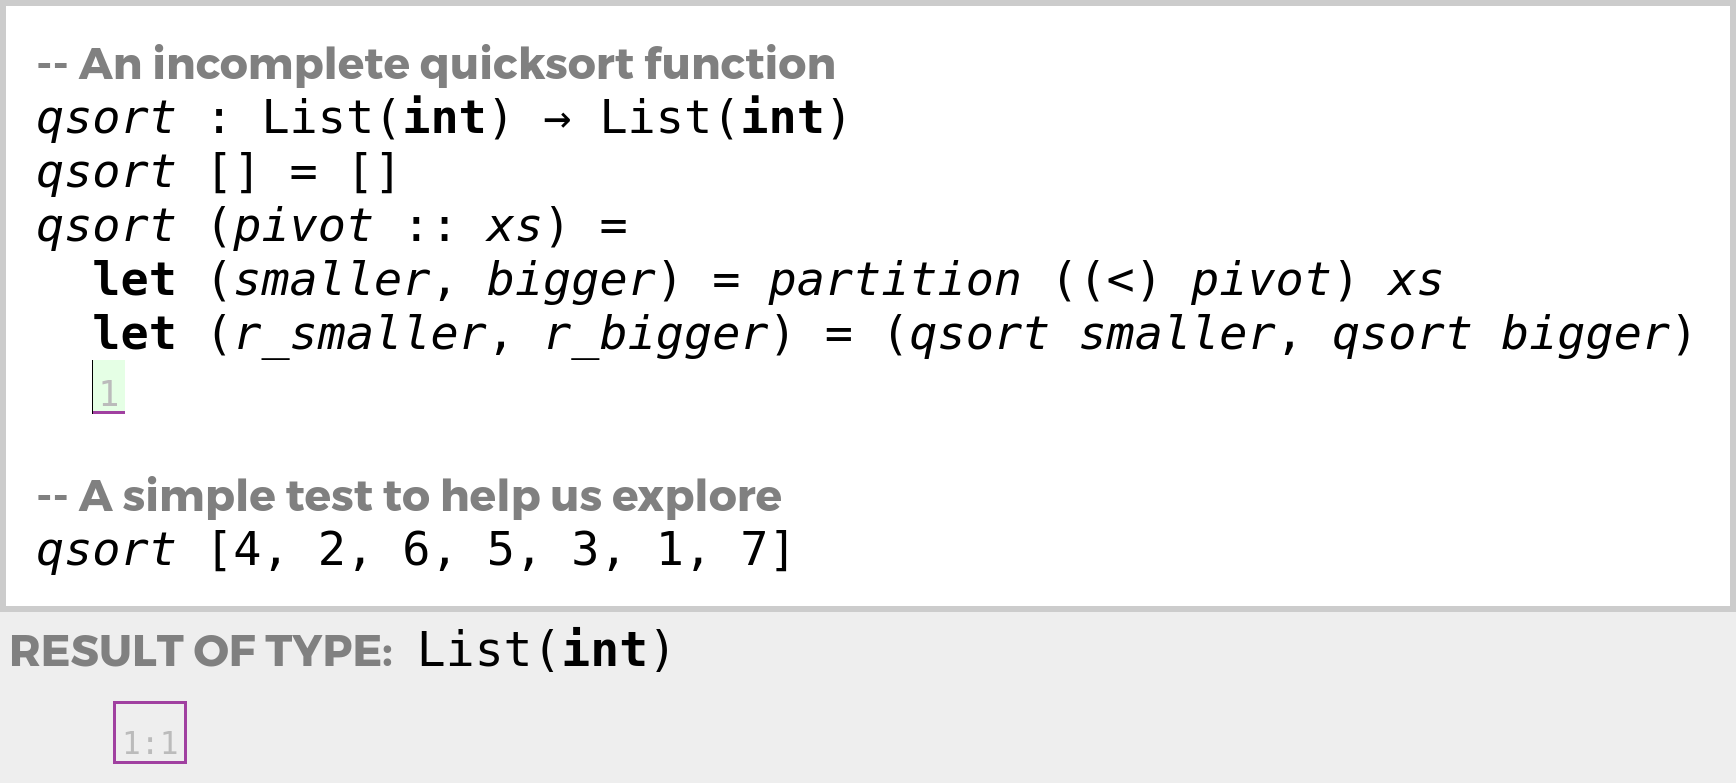
\includegraphics[width=\textwidth,interpolate=false,valign=t]{images/qsort-code.png}
\vspace{-3px}
\caption{The result of evaluation is a hole closure.}
\label{fig:qsort-example-code}
\end{subfigure}
~
\begin{subfigure}[t]{0.29\textwidth}
\centering
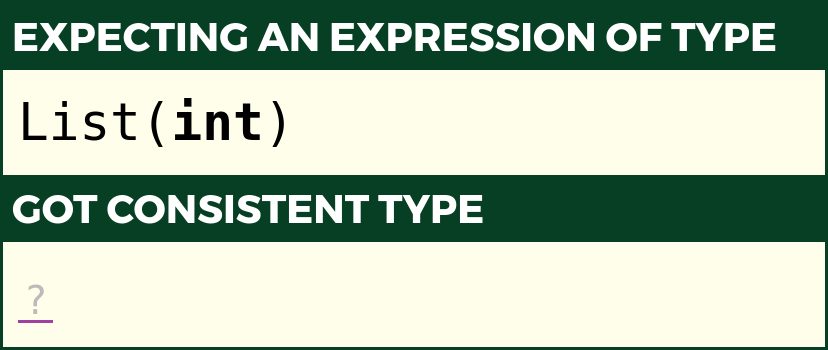
\includegraphics[width=\textwidth,interpolate=false,valign=t]{images/type-inspector.png}
\vspace{-3px}
\caption{The type inspector provides static feedback about the term at the cursor. Currently, the hole should be filled by a list expression. Holes have the hole (i.e. unknown) type, \li{?}, which  is universally consistent (see \cite{popl-paper,Siek06a}).
}
\label{fig:qsort-type-inspector}
\end{subfigure}

\vspace{8px}

\begin{subfigure}[t]{\textwidth}
\centering
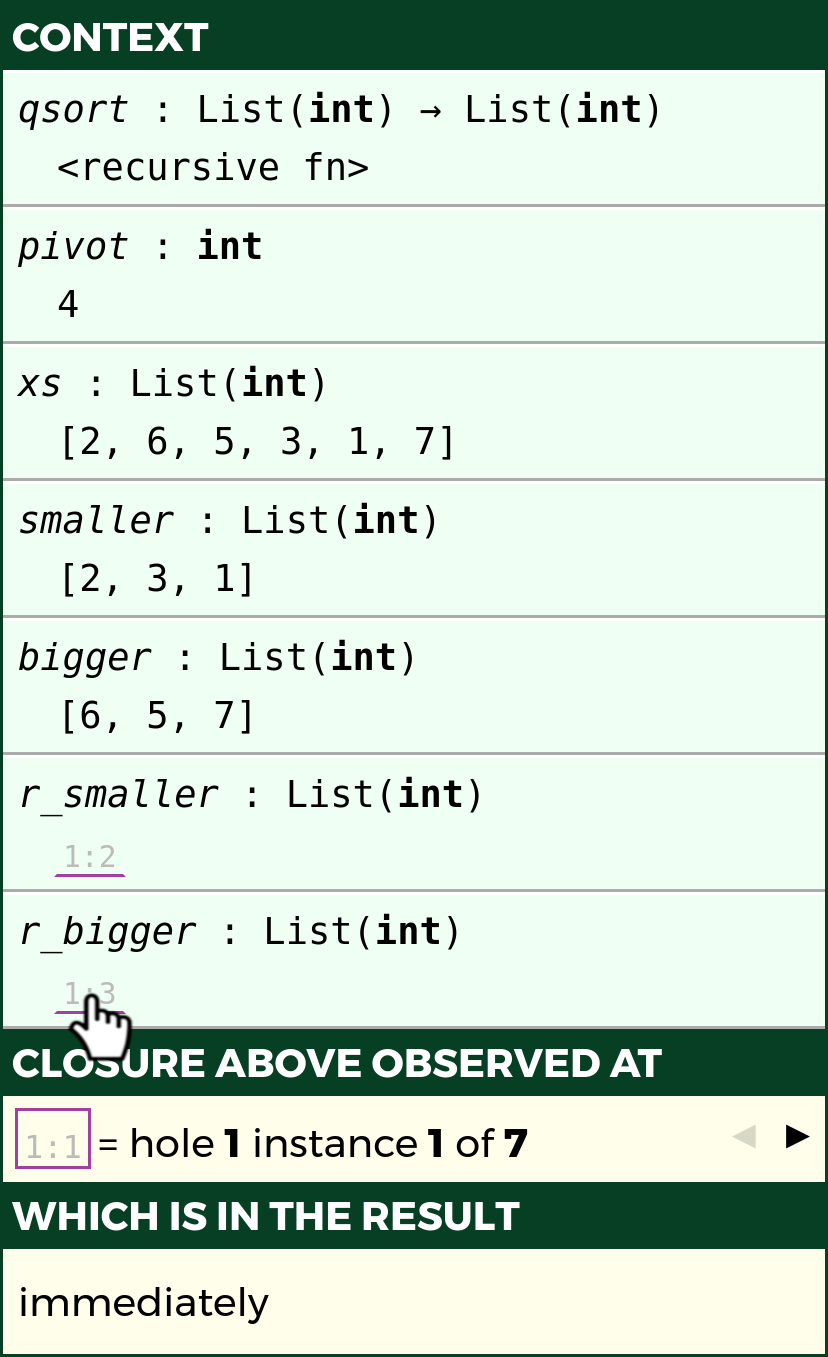
\includegraphics[width=0.29\textwidth,interpolate=false,valign=c]{images/qsort-new-sidebar-1.png}
~$\xrightarrow[\text{click}]{}$
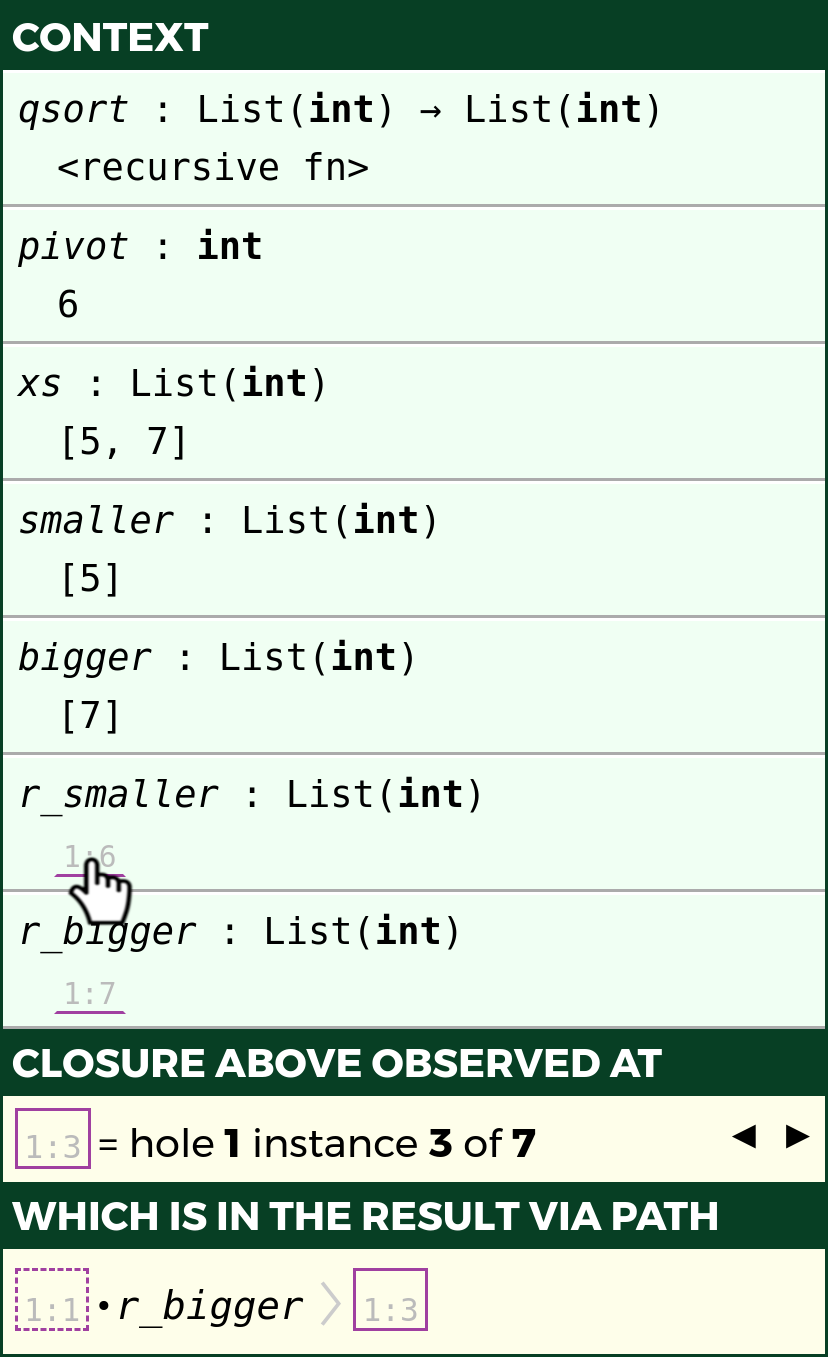
\includegraphics[width=0.29\textwidth,interpolate=false,valign=c]{images/qsort-new-sidebar-2.png}
~$\xrightarrow[\text{click}]{}$
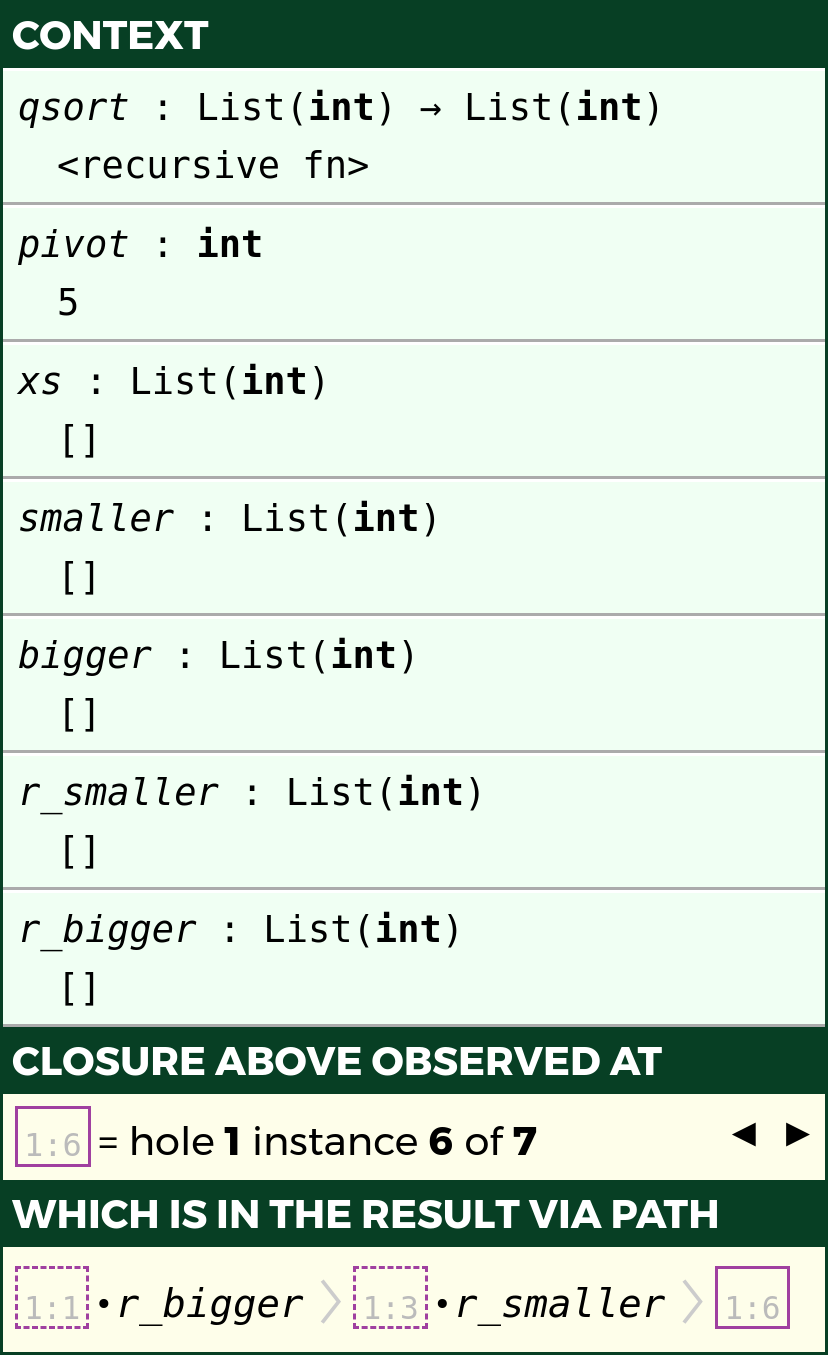
\includegraphics[width=0.29\textwidth,interpolate=false,valign=c]{images/qsort-new-sidebar-3.png}
\caption{The programmer can explore the recursive structure of the computation by clicking on hole instances.}
\label{fig:qsort-sidebars}
\end{subfigure}

\vspace{3px}

\caption{Example 1: Incomplete Quicksort}
\label{fig:qsort-cell-mockup}
% \end{subfigure}

\vspace{-5px}
\end{figure}

% \begin{subfigure}[t]{\textwidth}
% \centering
% 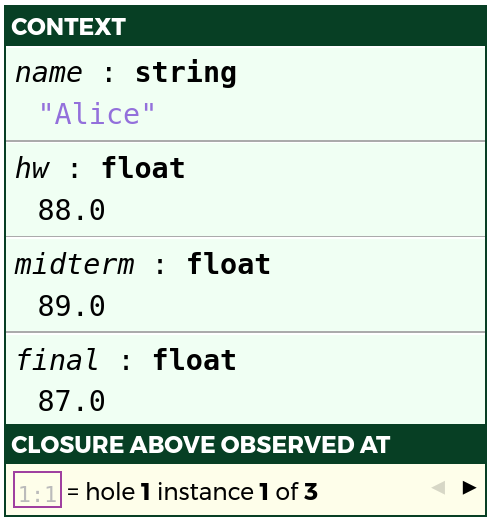
\includegraphics[width=0.3\textwidth,interpolate=false]{images/grades-sidebar-1.png}
% ~${}^\blacktriangleright$
% 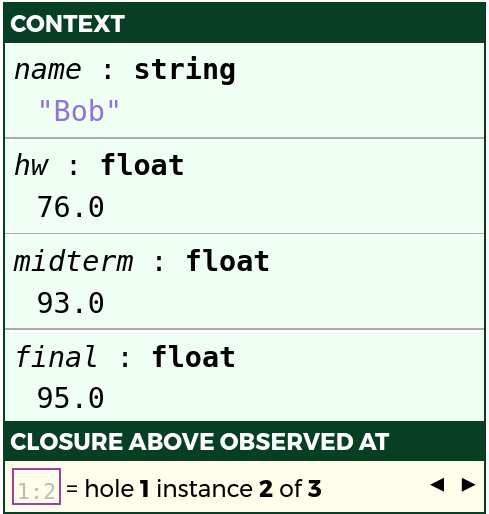
\includegraphics[width=0.3\textwidth,interpolate=false]{images/grades-sidebar-2.png}
% ~${}^\blacktriangleright$
% 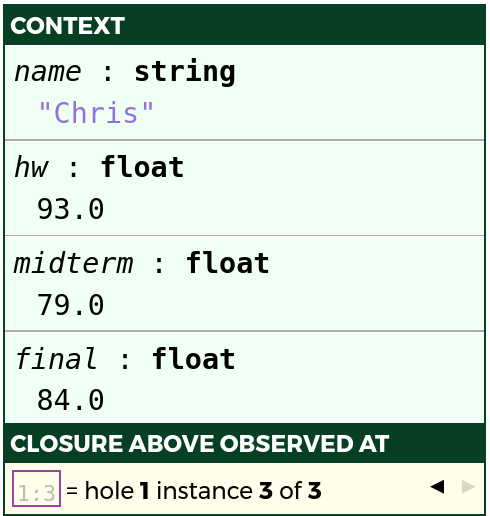
\includegraphics[width=0.3\textwidth,interpolate=false]{images/grades-sidebar-3.png}
% \caption{Typing context view with live hole closure information}
% \label{sec:grades-sidebar}
% \end{subfigure}
% %% TODO once the code above is removed, scale up the screenshots
% 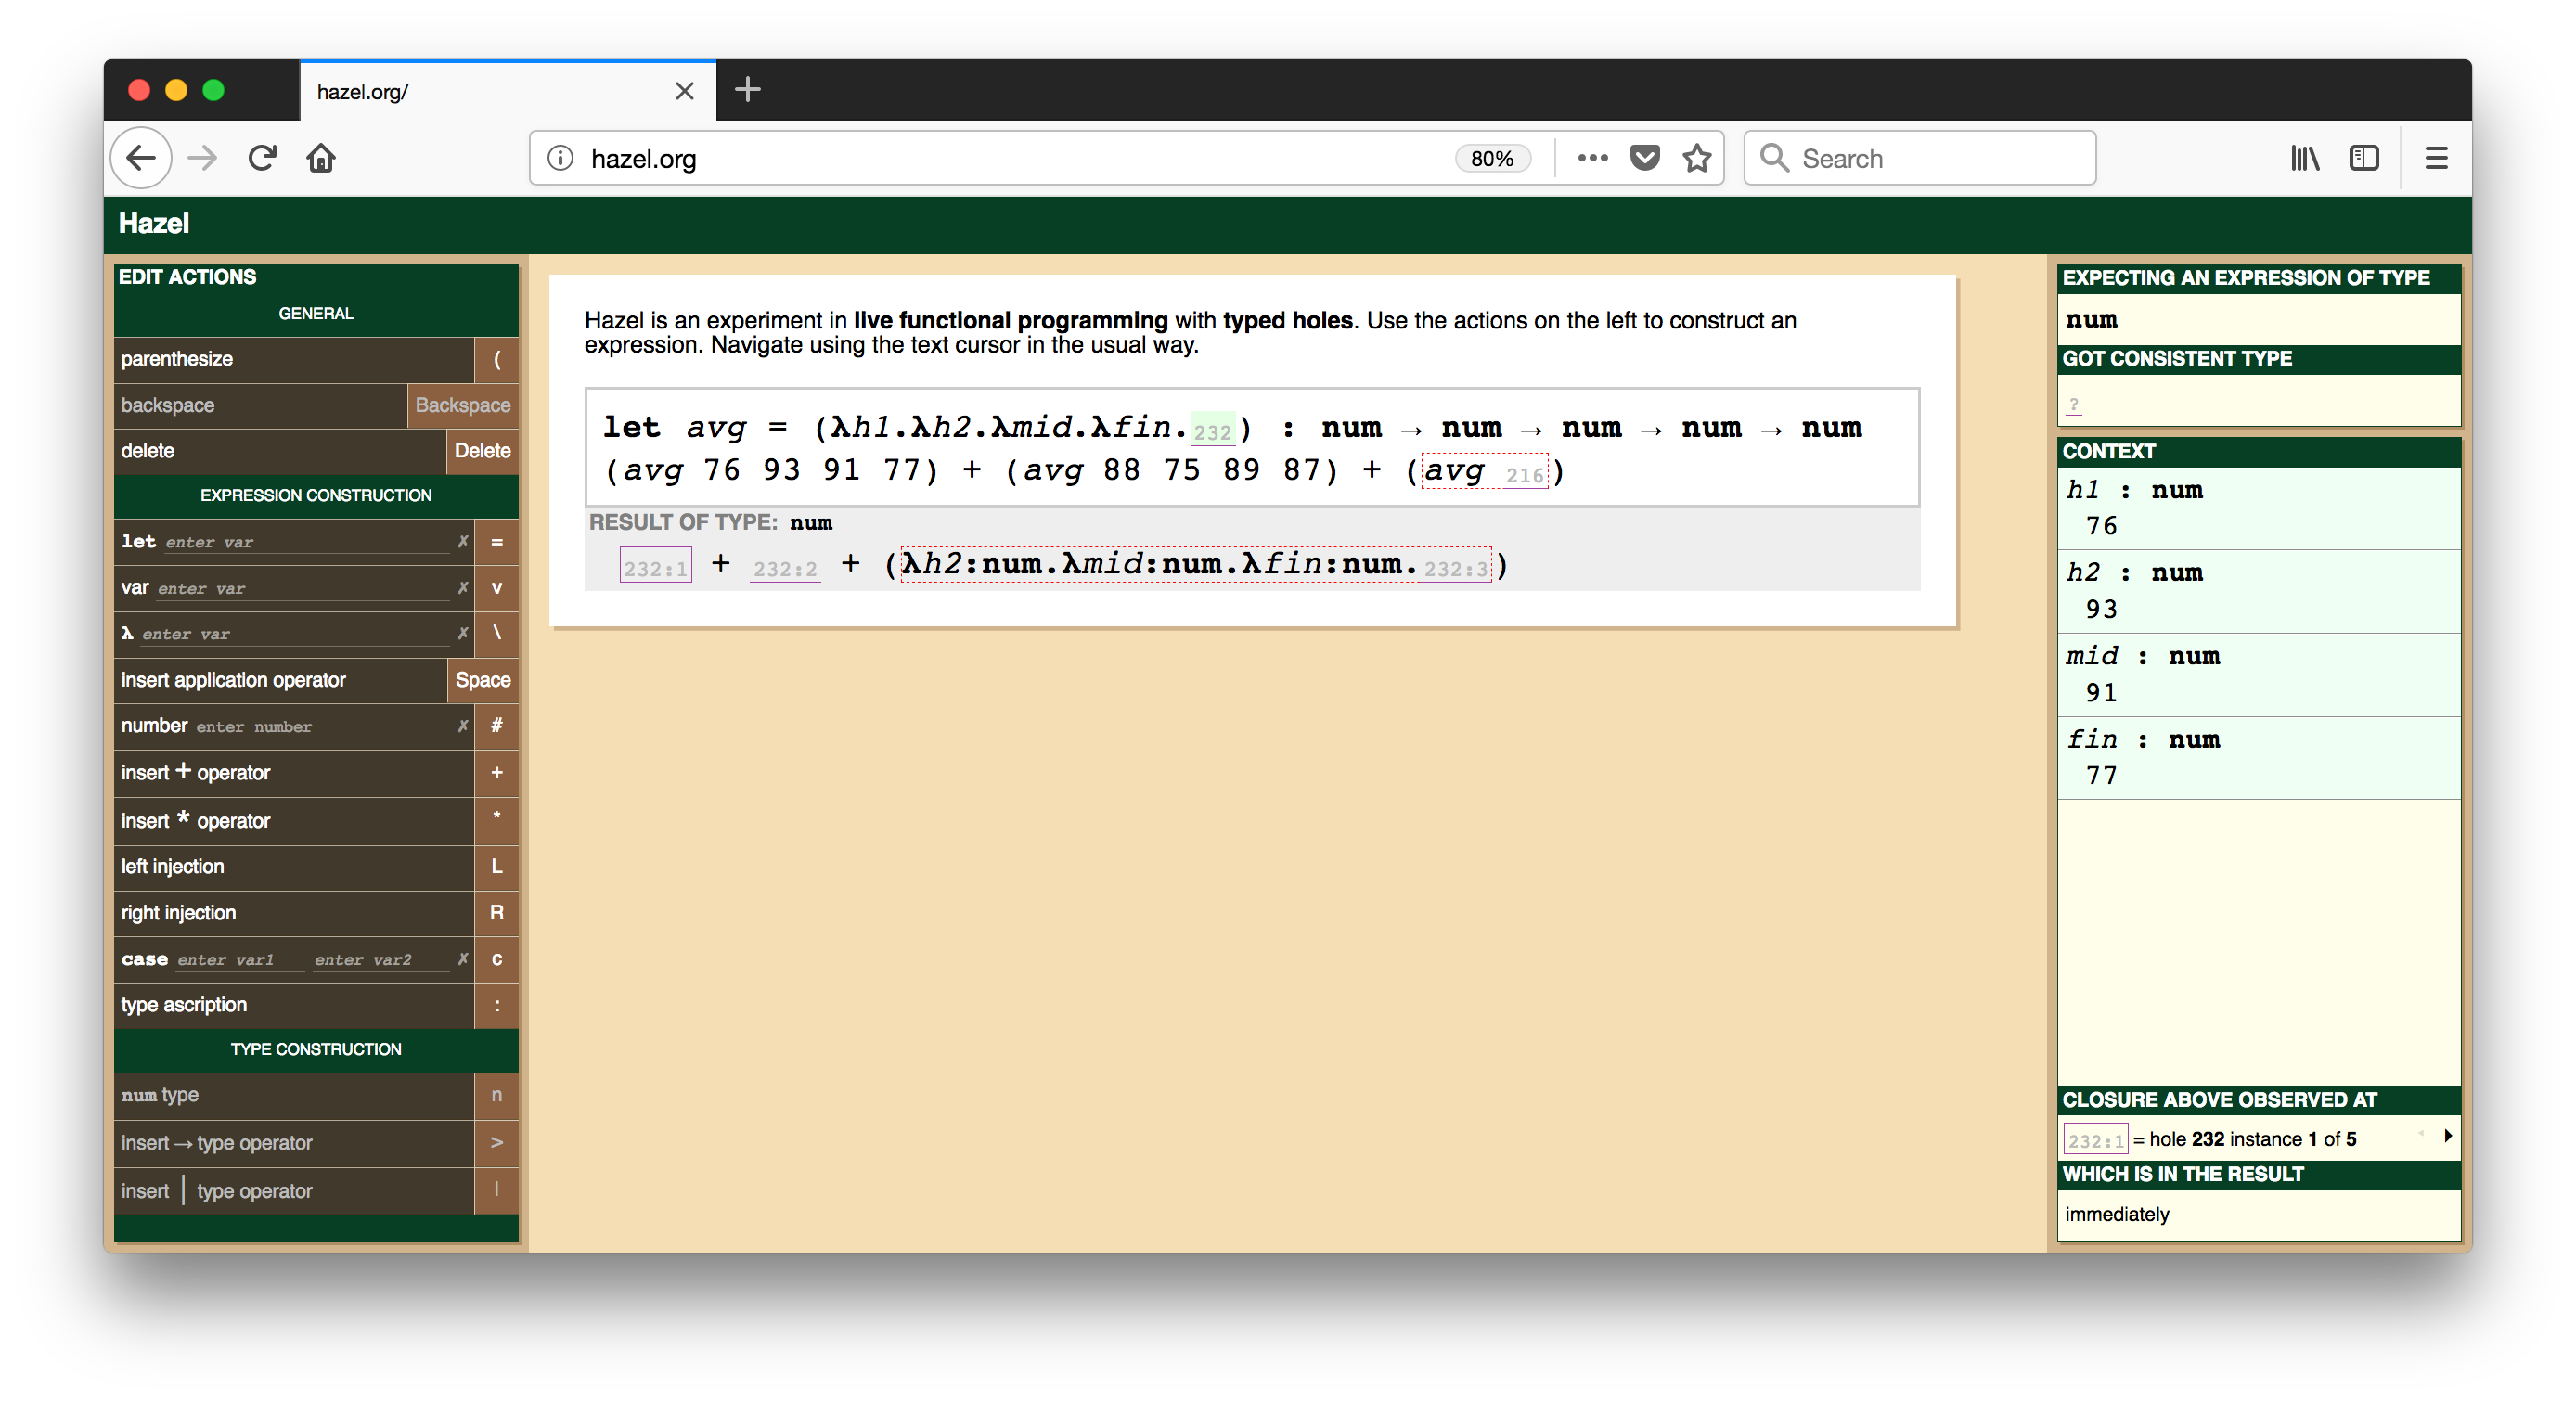
\includegraphics[scale=0.20]{images/hazel-placeholder-0.png}

% \rkc{Draw arrows and captions on the top figure to show how to get
% to the bottom figure.
% ser navigates to hole a, types + to create a plus, types * to create a
% multiplication, types \#10 to create 10, types vh1 to create variable use.}

% 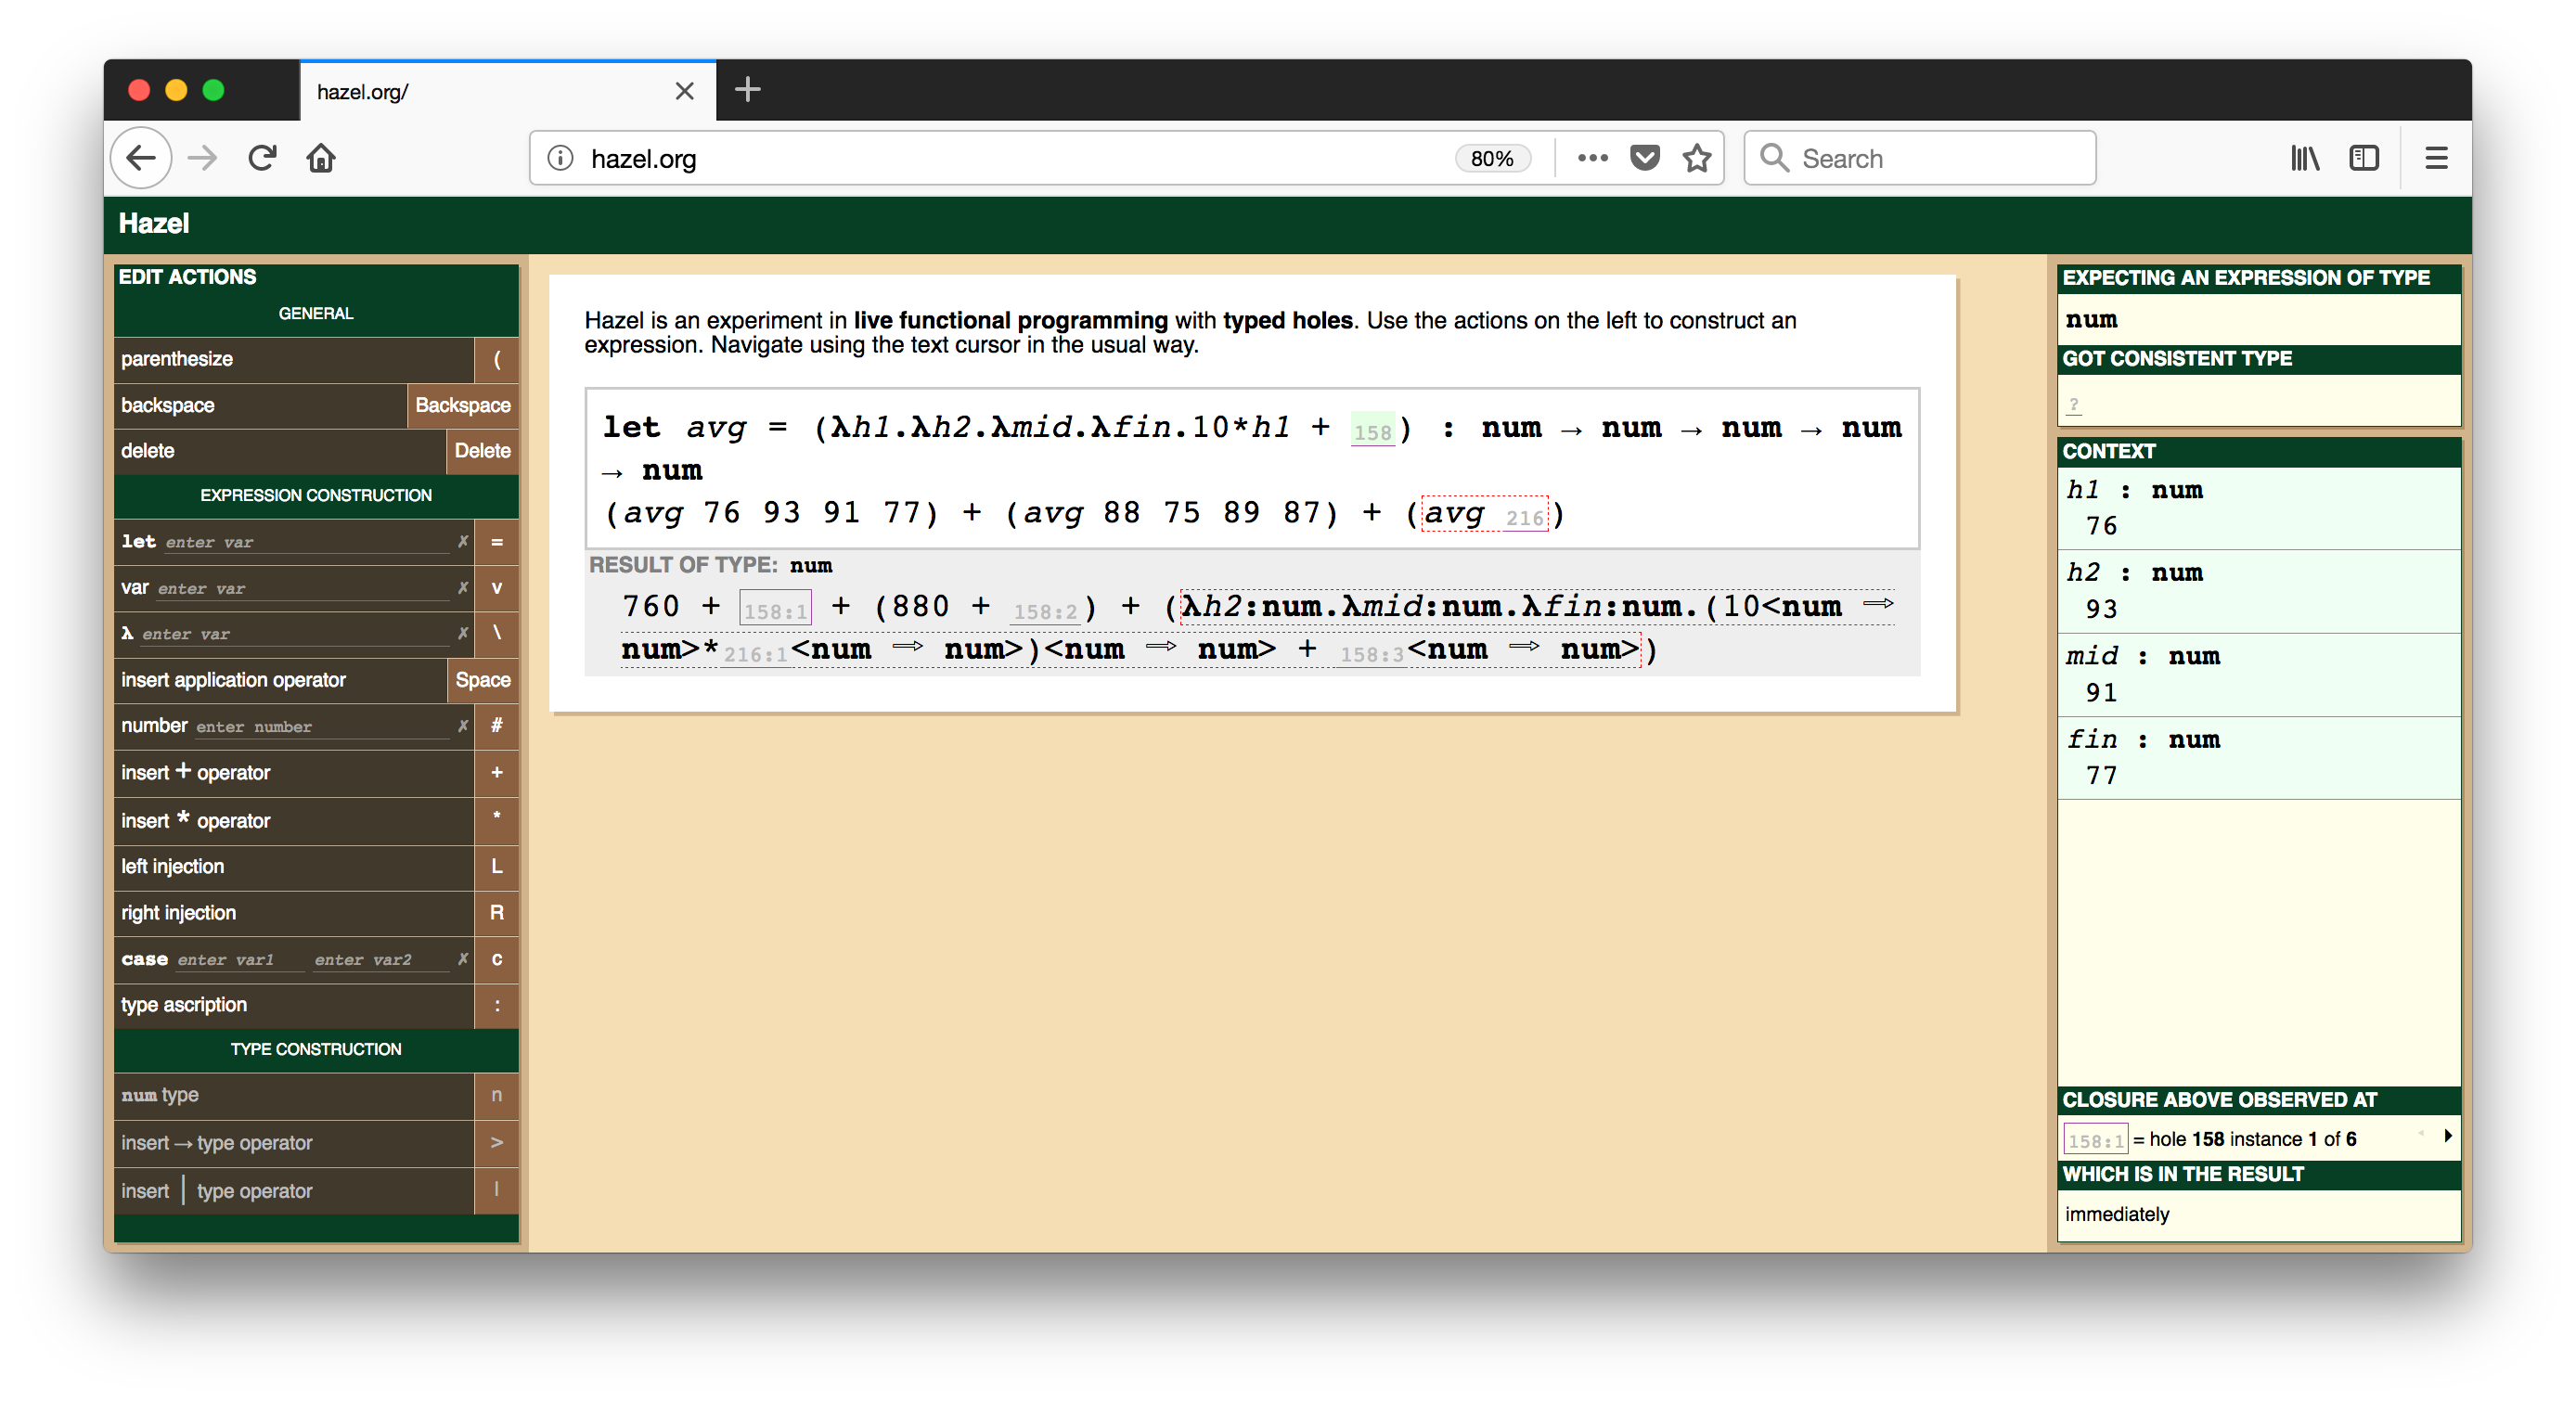
\includegraphics[scale=0.20]{images/hazel-placeholder-1a.png}


Let us now consider a second more sophisticated example: an incomplete implementation of the recursive quicksort function, shown in Fig.~\ref{fig:qsort-example-code}. So far, the programmer (perhaps a student, or a lecturer using \Hazel as a presentational aid) has filled in the base case, and in the recursive case, partitioned the remainder of the list relative to the head, and made the two recursive calls. A hole appears in return position as the programmer contemplates how to fill the hole with an appropriate expression of list type, as indicated by the \emph{type inspector} in Fig.~\ref{fig:qsort-type-inspector}.

At the bottom of the cell in Fig.~\ref{fig:qsort-example-code}, the programmer has applied \li{qsort} to an example list. However, 
the indeterminate result of this function application is simply an instance of hole \li{1}, which serves only to confirm that evaluation went through the recursive case of \li{qsort}. 
More interesting is the live context inspector, shown in three states in Fig.~\ref{fig:qsort-sidebars}, which provides feedback about the values of the variables in scope at hole \li{1} from the the various instances of hole \li{1} that appear in the result, either immediately or within an outer closure. For example, in its initial state (Fig.~\ref{fig:qsort-sidebars}, left) it shows the closure at the instance of hole \li{1} that appears immediately in the result due to the outermost application of \li{qsort}. From this, the programmer can confirm (or the lecturer can visually point out) that 
the lists \li{smaller} and \li{bigger} computed by the call to \li{partition} are appropriately named, and observe that they are not yet themselves sorted.

The results from the subsequent recursive calls, \li{r_smaller} and \li{r_bigger}, are again hole instances, \li{1:2} and \li{1:3}. 
The programmer can click on either of these hole instances to reveal the associated closures from the corresponding recursive calls. 
For example, clicking on \li{1:3} reveals the hole closure from the \li{r_bigger} recursive call as shown in Fig.~\ref{fig:qsort-sidebars} (middle). 
From there, the programmer can click another hole closure, e.g. \li{1:6} to reveal the hole closure from the subsequent \li{r_smaller} recursive call as shown in Fig.~\ref{fig:qsort-sidebars} (right). 
Notice in each case that the path from the result to the selected hole closure is reported as shown at the bottom of the context inspector in Fig.~\ref{fig:qsort-sidebars}. 
In exploring these paths rooted at the result, the programmer can develop concrete intuitions about the recursive structure of the computation (e.g. by following through to the base case as shown in Fig.~\ref{fig:qsort-sidebars}) even before the program is complete. 
% (We leave to future work the pedagogical question of whether such early feedback might help students understand recursion.)

\begin{comment}
Now the teacher returns to \lismall{weighted_average} to work on the missing
expression, with the goal of computing a weighted sum of each of a student's
grades.
%
The teacher performs several \Hazel{} edit actions (each of which is a single
keystroke, a shortcut to selecting one of the edit tools from the left panel,
followed by a tool-specific argument terminated with the Enter key):
%
navigating the cursor to hole \lismall{a} and typing \lismall{+}, which creates a
sum expression \lismall{??_b + ??_c} with the cursor placed, by default, under
left operand (the hole labeled \lismall{b});
%
typing \lismall{*} to create a multiplication expression \lismall{??_d * ??_e + ??_c},
with the cursor place under hole \lismall{d};
%
typing \lismall{\#10} to enter a numeric scaling factor, which then moves
the cursor to the second operand, hole \lismall{e}; and
%
typing \lismall{vg.hw1} to use the \lismall{hw1} field of the function argument
as the right operand of the multiplication.
%
The resulting partial expression, \lismall{(10.0 *. g.hw1) +. ??_b}---shown
in the screenshot in the bottom half of \autoref{fig:grades-example}---marks the
first of five weighted summands in the eventual finished \lismall{weighted_average}
calculation.
\end{comment}

\begin{comment}
Each \Hazel{} edit action transforms an incomplete but well-formed and
well-typed program into another such program, and, thus, \Hazel{} immediately
runs the program after each edit.
%
After the above edit sequence, \Hazel{} display the updated list of
indeterminate expressions \lismall{[760.0 + ??_b.1, 880.0 + ??_b.2, ...]}.
%
Right away, the teacher recognizes that the values are too large; they should be
at most \lismall{100.0}.
%
The teacher realizes that representing percentage points as \lismall{float}s requires
that the constant on line \rkc{XXX} ought to be \lismall{0.10} instead.
%
Because of this live feedback, the teacher corrects this error right away and
avoids making similar programming errors in the rest of the calculation.
%
The teacher continues to build the rest of the arithmetic expression until it is
complete (there are no longer any expression holes), and the result of
immediately running the finished program shows that each of values in the final
result list is in the range \lismall{0.0} to \lismall{100.0}.
\end{comment}

\begin{comment}
\begin{figure}[t]

\rkc{Move all this code into the mockup screenshots below.}

\lstset{basicstyle=\scriptsize\ttfamily}
\begin{lstlisting}
type grade_cutoffs =
  { a: float, b: float, c: float, d: float, f: float };

let cutoffs =
  { a = ??_a, b = ??_b, c = ??_c, d = ??_d, f = ??_f };

let letter_grade(n: weighted_average) =
  if n >= cutoffs.a then "A" else
  if n >= cutoffs.b then "B" else
  if n >= cutoffs.c then "C" else
  if n >= cutoffs.d then "D" else
  if n >= cutoffs.f then "F" else "Incomplete";

let sorted_weighted_averages = List.sort weighted_averages;

let letter_grades = List.map letter_grade sorted_weighted_averages;

let compute_distribution(list: list(float)) =
  let n = List.length letter_grades in
  List.map
    (\x -> (x, showPercentage (List.length (List.filter ((==) x) list)) /. n))
    ["A","B","C","D","F","Incomplete"];

let distribution = compute_distribution(letter_grades);
\end{lstlisting}
%% restore settings from main.tex
\lstset{basicstyle=\footnotesize\ttfamily}

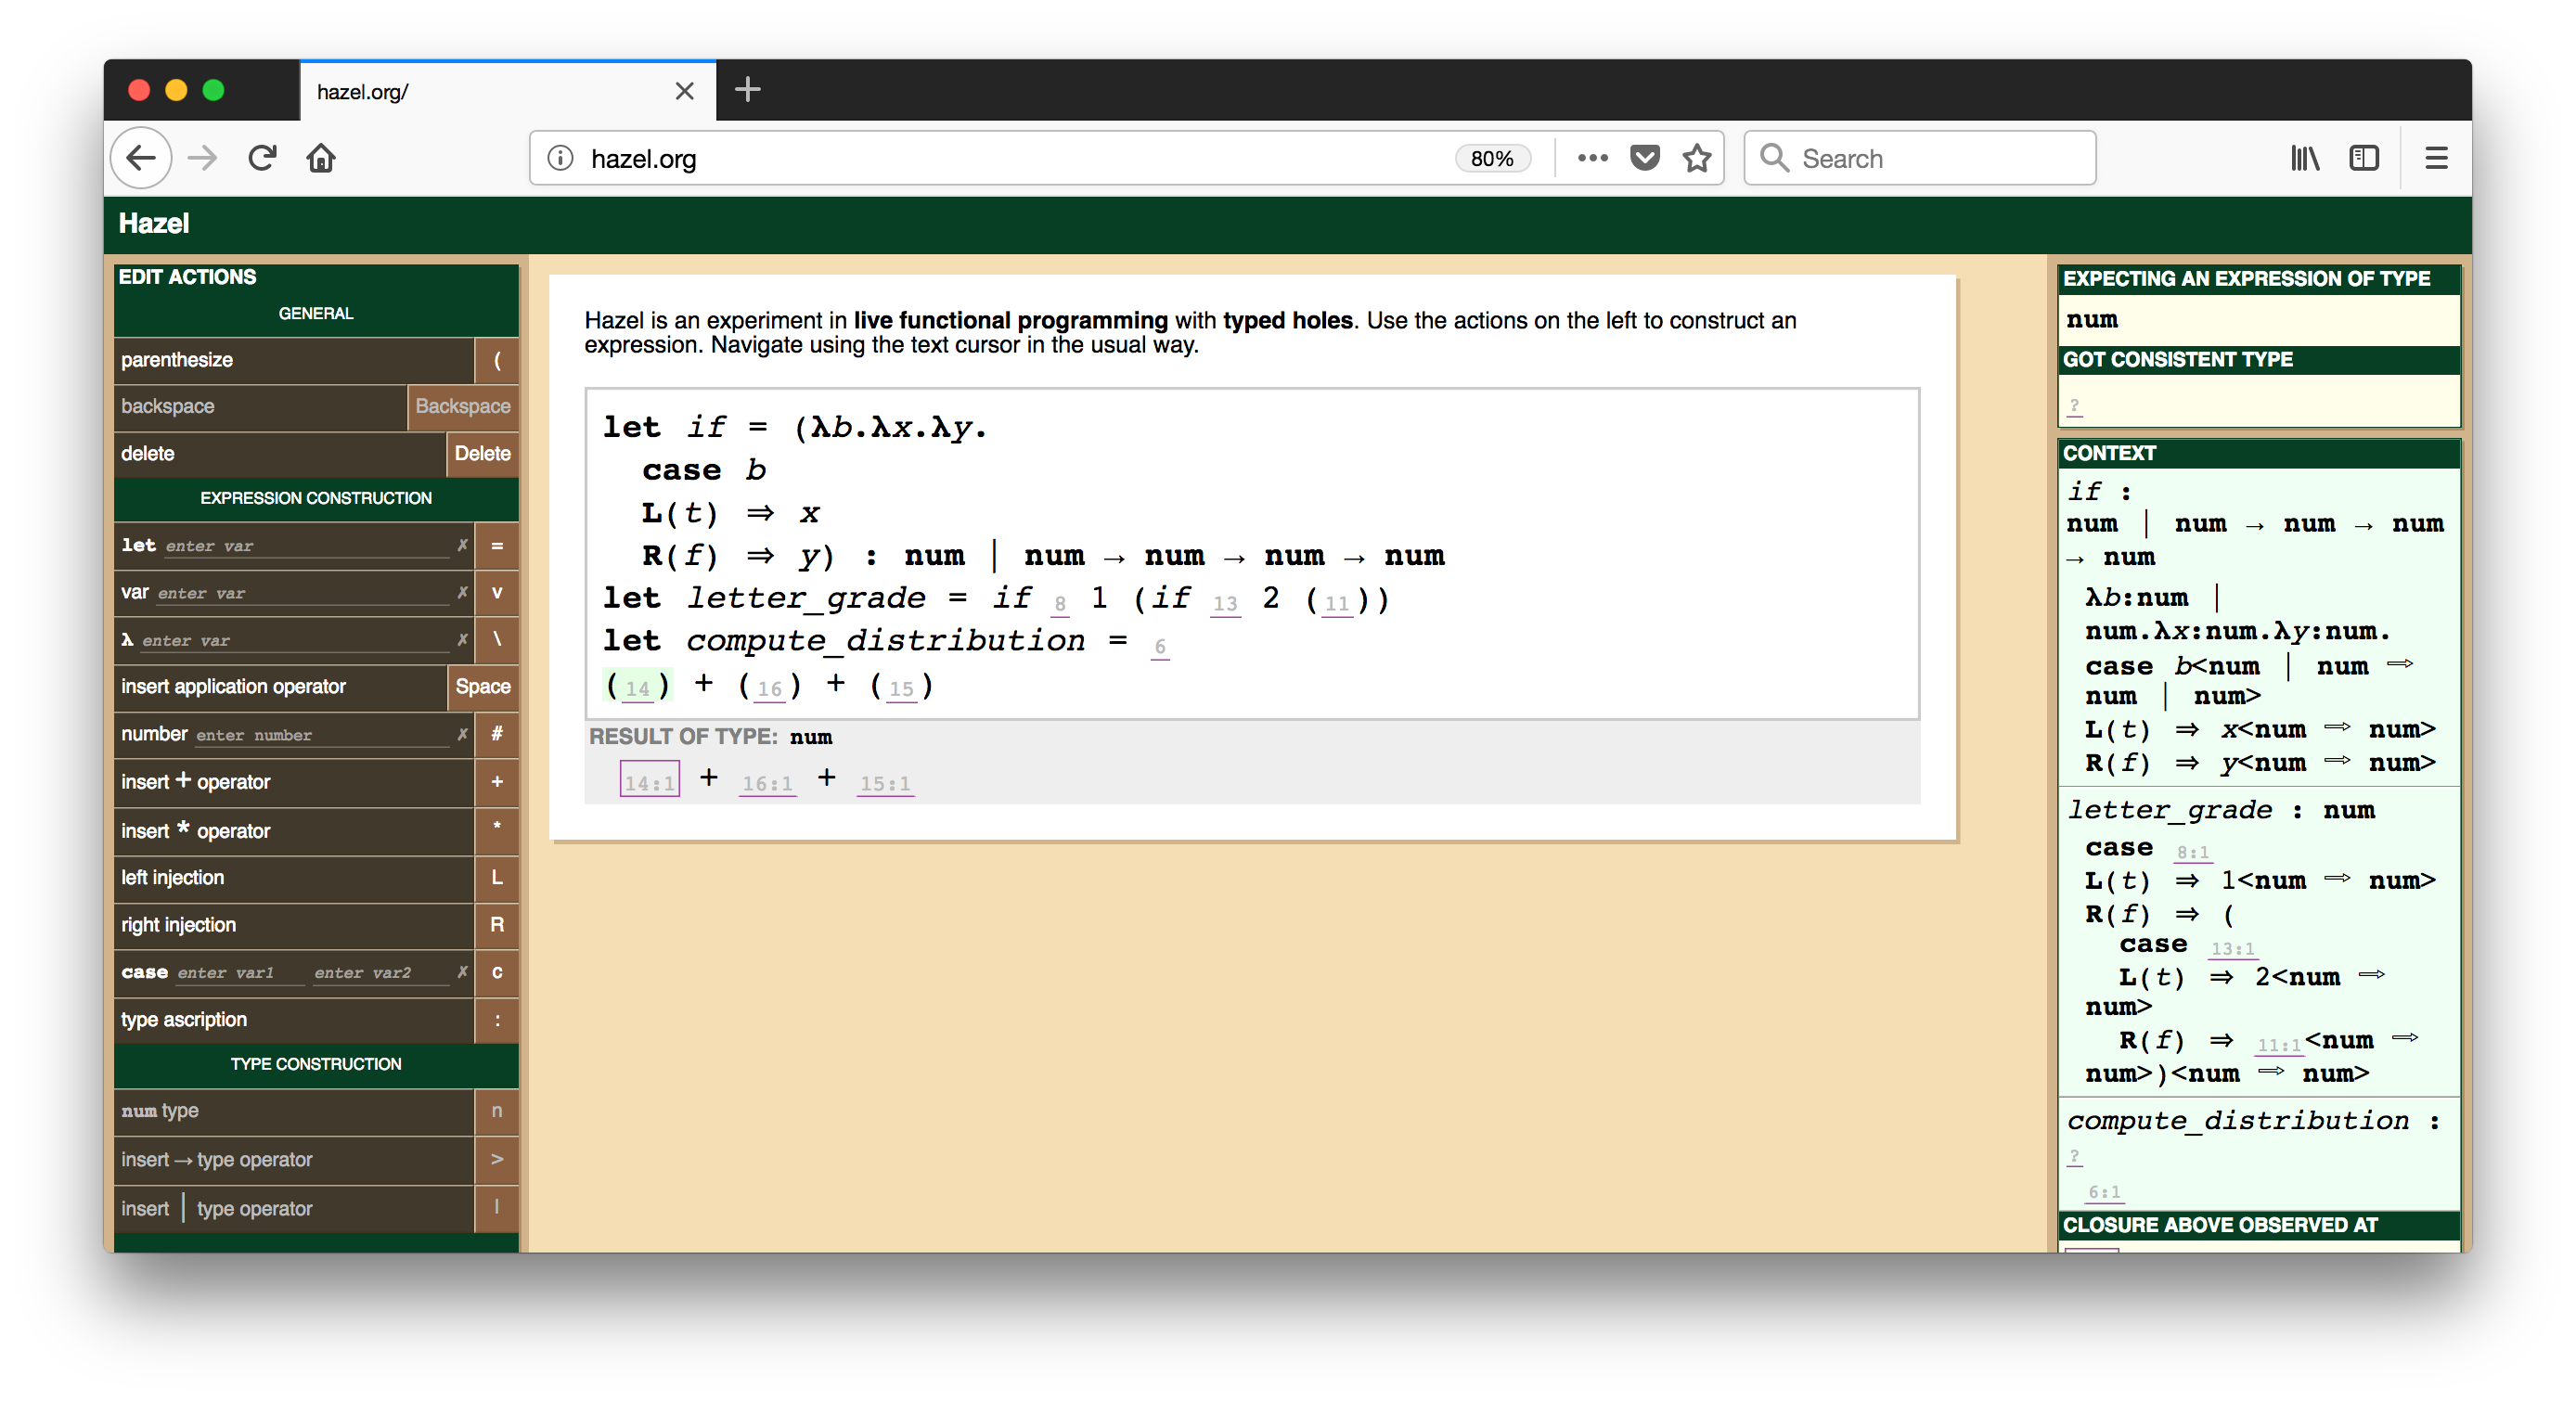
\includegraphics[scale=0.27]{images/hazel-placeholder-1b.png}

\caption{Hazel mockup for Example 1b.}
\label{fig:grades-example-b}
\end{figure}


\overviewExample{1b}{Assigning Letter Grades}
%
The teacher's next task is to map the weighted averages to the letter grades A
through F (we consider only ``whole'' letter grades, for simplicity).
%
The \lismall{grade_cutoffs} record type, shown at the top of
\autoref{fig:grades-example-b}, describes the minimum cutoff for each of
these six possible grades.
%
Initially, each value in the \lismall{cutoffs} record is a hole.

%
%% initially all holes, because it will be different year-to-year based on the %
%data, differences in course difficulty, and to satisfy fairness criteria.
%
Before starting to fill in the cutoff values, the teacher jumps ahead to write a
function \lismall{letter_grade} that will make the connection between \lismall{cutoffs}
and \lismall{weighted_averages}.
%
Because she intends to look at the data to help select the cutoff values, the
teacher sorts the \lismall{weighted_averages} (on line \rkc{XXX}) and then maps
them to \lismall{letter_grades} (on line \rkc{XXX}).

When \Hazel{} runs this program, the guard of the outermost conditional
(\lismall{n >= cutoffs.a} on line \rkc{XXX}), is indeterminate because \lismall{cutoffs.a}
is.
%
Therefore, each of the indeterminate expressions in \lismall{letter_grades} is the
entire expression body, albeit with different bindings for \lismall{n}.
%
Displaying such ``large'' indeterminate expressions can quickly consume all
available screen space, overwhelming the user with too much information.
%
\autoref{fig:XXX} shows how \Hazel{} renders large indeterminate
expressions (\ie{}~anything other than ``small'' indeterminate value (a constant
or hole) or list of small values) simply as \lismall{..} to save space.
%
Hovering over this abbreviation (\rkc{???}) displays the full
indeterminate expression---as well as the evaluation environment that surrounds
it---as a tooltip.
%
\autoref{sec:discussion} discusses this and other user interface concerns when
trying to display useful live feedback without overwhelming the user.
%
These usability factors are beyond the scope of our work, which is to define
semantic foundations on which such user interfaces can be built.

To start deciding \lismall{cutoffs}, the teacher clicks the \lismall{weighted_averages}
expression, and views the results panel to see the data sorted in descending
order.
%
The result shows a natural gap between \lismall{92.2} and \lismall{89.5}.
%
So, she chooses to use \lismall{92.0} as the cutoff for A, replacing hole \lismall{XXX} on
line \rkc{XXX} with that numeric value.
%
Resuming the computation from before, \Hazel{} resolves the conditional
expressions for the first \rkc{XXX} indeterminate expressions, because each of
those \lismall{n} values was greater than \lismall{cutoffs.a}.
%
The remaining \rkc{XXX} expressions also proceeded to evaluate the first guard,
and are now indeterminate at the guard for the second conditional.

Before assigning subsequent cutoff values, the teacher would like to get a sense
of whether this first choice is a good one.
%
She jumps ahead to to write a function (\lismall{compute_distribution} on lines
rkc{XXX}-\rkc{XXX}) that computes the distribution of letter grades based
on \verb+cutoffs+..
%
Running \lismall{compute_distribution} shows that the percentage of As is
\rkc{XXX\%}, which is smaller than what the teacher would like;
the remaining percentages are all indeterminate.
%
Returning to the value of \lismall{sorted_data}, she sees a cluster around \lismall{89.0}
and then another gap between \lismall{88.2} and {85.5}.
%
So, the teacher adjusts \lismall{cutoffs.a} to be \lismall{88.0}.
%
Because this edit is not just filling a hole expression, \Hazel{} discards the
previous execution state and reevaluates the entire program.
%
Existing techniques for incremental computation~\cite{XXX,XXX}, however, could
be applied to seek opportunities for reuse even when non-hole expressions are
modified.
%
Because the focus of work is on the novel implications of running programs with
holes, our calculus and implementation supports caching ``edit-and-resume'' only
for the novel situation in which evaluation proceeds around holes.
%
After re-evaluation, the percentage of As becomes \rkc{XXX\%}, which better
matches the teacher's intention.

In this fashion, the teacher continues down the list of sorted averages,
determining appropriate values for each cutoff.
%
Whenever the teacher is only filling in the ``next'' cutoff, the computation
from before can simply be resumed.
%
Overall, throughout the workflow described in these two examples, the programmer
can continue to evaluate the program, and receive meaningful feedback, while
going back and forth between different pieces under development.
\end{comment}

% !TEX root = hazel-LIVE2018.tex

%% \subsection{Live Programming with Type Errors}

\subsection{Example 2: Live Programming with Static Type Errors}
\label{sec:static-errors}


% \begin{subfigure}[t]{\textwidth}
\begin{figure}
\centering
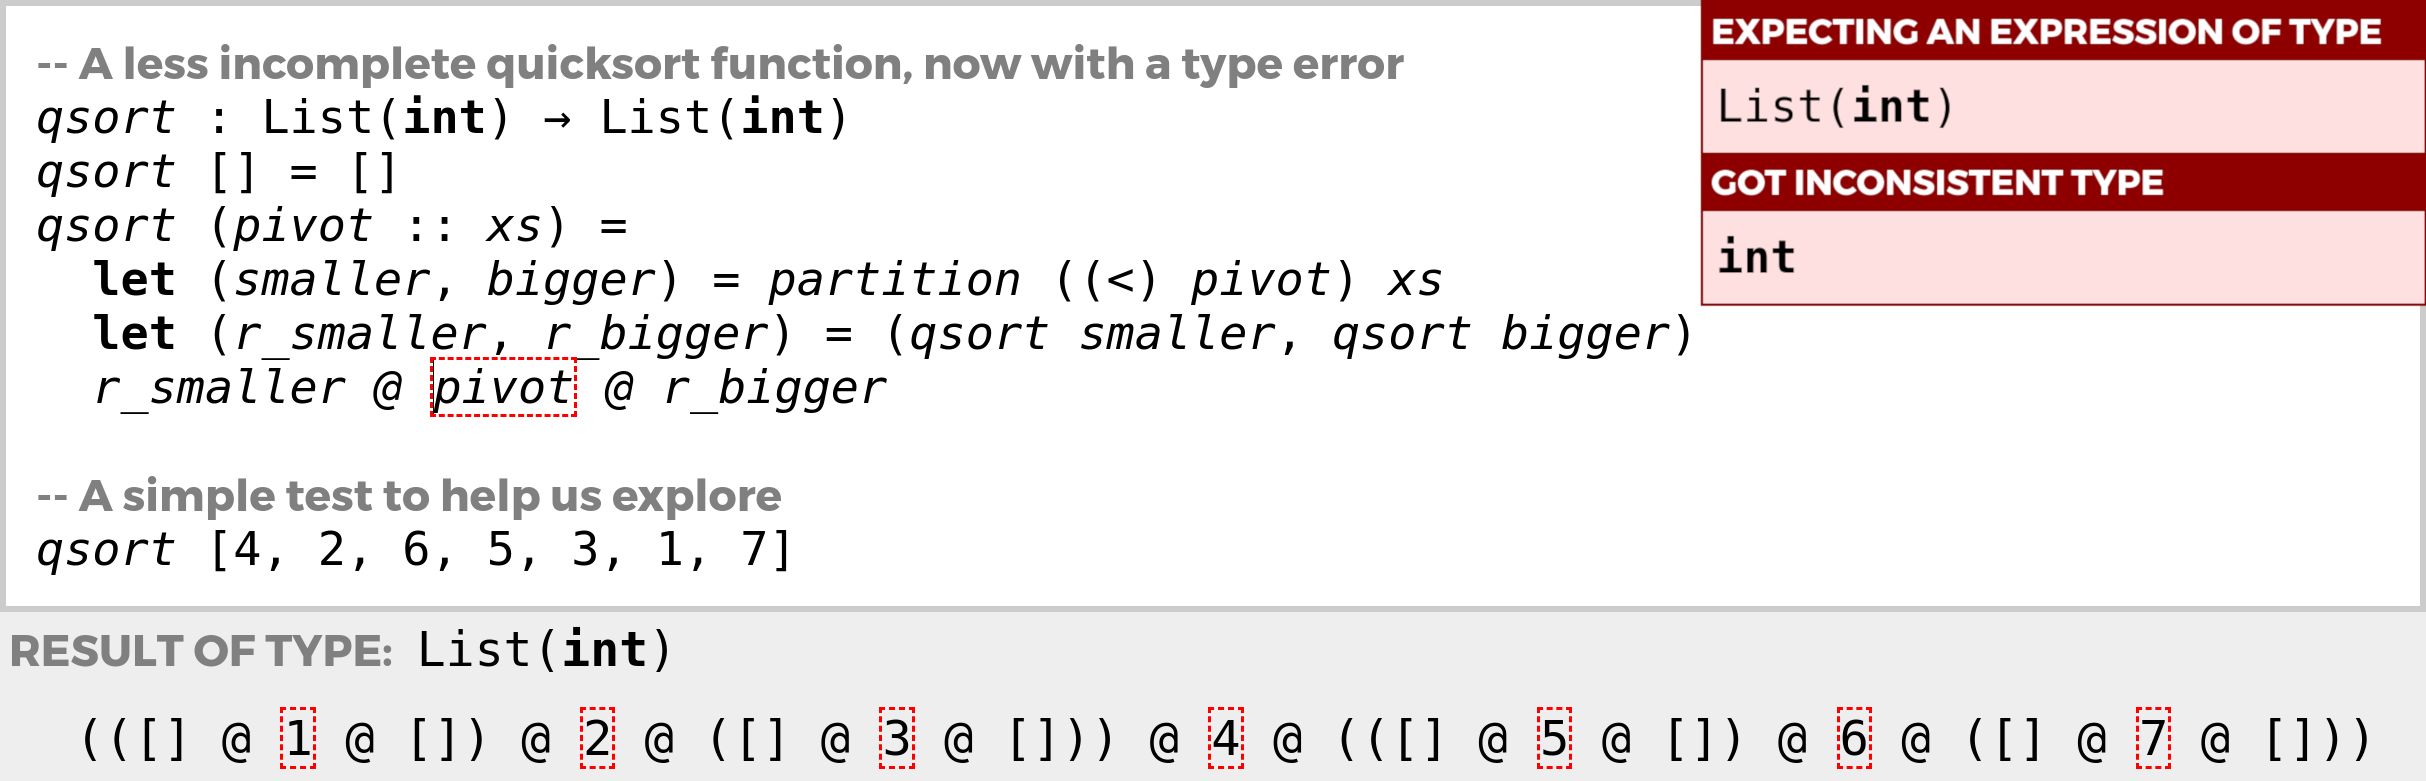
\includegraphics[width=0.96\textwidth,interpolate=false,valign=t]{images/qsort-type-error-inset.png}
% 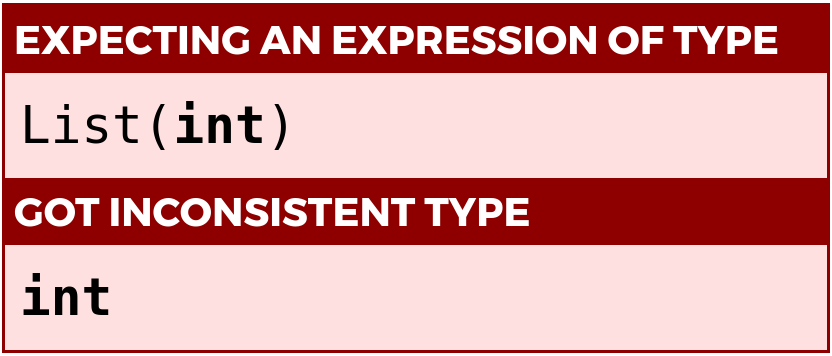
\includegraphics[width=0.28\textwidth,interpolate=false,valign=t]{images/type-inconsistency.png}
\caption{Example 2: Ill-Typed Quicksort}
\label{fig:qsort-type-error}
\vspace{-4px}
\end{figure}
% \end{subfigure}


The previous example was incomplete 
because of \emph{missing} expressions.
%
Now, we discuss programs that are incomplete, 
and therefore conventionally meaningless, because of
\emph{type inconsistencies}. In particular, 
%
let us 
assume that the programmer has filled in hole \li{1} in the previous example 
as shown in Fig.~\ref{fig:qsort-type-error}. 
The result computed in Fig.~\ref{fig:qsort-example-code} recorded the environment around every
instance of hole \li{1}, so the new result can be computed from the previous result by performing 
contextual substitution (a concept from contextual modal type theory \cite{Nanevski2008})  and resuming evaluation, rather than restarting evaluation entirely.
For larger examples, this \emph{fill-and-resume} operation could significantly reduce evaluation time, which is  
important to perceived liveness \cite{DBLP:conf/icse/Tanimoto13}. 

The programmer appears to be on the right track conceptually
in recognizing that the pivot needs to appear between the 
smaller and bigger elements. 
However, the types do not quite work out: the \li{@} operator here
performs list concatenation, but the pivot is an integer. 
Most compilers and editors will report a static error message
to the programmer in this case, and \Hazel 
follows suit in the type inspector (shown inset in Fig.~\ref{fig:qsort-type-error}). 
However, our argument is that the presence of a static type error should not cause all feedback about 
the dynamic behavior of the program to ``flicker out'' or ``go stale'' --
after all, there are perfectly meaningful parts of the program (both nearby
and far away from the error) 
whose dynamic behavior may be of interest. Evaluation can also assist the programmer in understanding the type error by presenting concrete values \cite{Seidel2016}.
% After all,
% the error is localized and there is perfectly good code elsewhere 
% in the program (if not nearby, then perhaps far away).

Our approach, following the prior work of \citet{popl-paper}, 
is to semantically internalize the ``red outline'' around
a type inconsistency, representing it as a \emph{non-empty hole}.
Evaluation safely proceeds past a non-empty hole just as if it were an empty hole.
Evaluation proceeds inside the hole, so that 
feedback about the type-inconsistent expression, which might ``almost'' be correct, is available. 
In this case, the result at the bottom of Fig.~\ref{fig:qsort-type-error}
reveals concretely that the programmer is on the right track: the list elements 
appear in the correct order.
They simply have not been combined correctly. 
The semantics also associates an environment with each instance of a non-empty hole,
so we can use the live context inspector essentially as in Fig.~\ref{fig:qsort-sidebars} (not shown). 


% For example, consider the following two definitions.

% \begin{lstlisting}
% let bad_bool : bool = ?? 0 ??_bad_bool;

% let bad_int : int = 1 + ?? true ??_bad_int_second_argument;
% \end{lstlisting}

% \noindent
% %
% These two definitions are ill-typed under standard typing disciplines.
% %
% In contrast, \citet{popl-paper} present a bidirectional type system that assigns
% types to both, by wrapping type-inconsistent expressions (\li{0} on line
% \rkc{XXX} and \li{true} on line \rkc{XXX} above) in \emph{non-empty} holes.
% %
% Non-empty holes prevent local type inconsistencies from polluting the rest of
% the program surrounding it, which may or may not itself contain additional
% inconsistencies.

\begin{comment}
\overviewExample{2}{Sum List}
%
Consider the following buggy program (observed during an undergraduate
functional programming course~\cite{Seidel2016}) that attempts to sum a list
integers.
%
The error is that the base case produces a list rather than an integer.

\begin{lstlisting}
sum_list : list(int) -> int
sum_list [] = ?[]?
sum_list (n:ns) = n + sum_list ns
\end{lstlisting}

\noindent
%
Because the list expression on line 2 does not have type \li{int} as required,
it is wrapped in a (non-empty) hole by the bidirectional type
checker~\cite{popl-paper}.
%
Rather than trying to debug the error based on the static error, the programmer
may wish to trying running the function anyway by calling, say, \li{sum_list(2)}.
%
\HazelnutLive{} runs and produces the indeterminate expression \li{3 + ?[]?}.
%
By observing that the hole expression is being added to the integer \li{3}, he
realizes that it needs to be an integer, specifically, \li{0}.
%
Compared to the trace displayed by \citet{Seidel2016}, the indeterminate result
produced by \HazelnutLive{} is ``flattened'' because the expression \li{1 + 2}
successfully proceeded to evaluate despite the error elsewhere.
\end{comment}

%% TODO fold error from Erwig paper.
%% %
%% see that final call on stack does have the right answer, but
%% it's wrapped in a singleton list when the expected type is not
%% a list.
%% %
%% fix is to remove the list, the rest of the computation remains
%% the same, but b/c they were all wrapped in holes, need to re-run.
%% %
%% (add some mechanism for type-consistent non-empty-holes...)

\begin{comment}

\overviewExample{4}{Stutter}
%
Consider the following function which attempts to produce a
list where every element is repeated twice (borrowed from \citet{Osera2015}).
%
The combiner function to \li{List.foldr} needs to produce a \li{list(int)}, but
it produces a \li{list(list(int)} instead.

\begin{lstlisting}
stutter : list(int) -> list(int)
stutter xs = List.foldr (\x acc -> ?[x,x]? : acc) [] xs
\end{lstlisting}

\noindent
%
The bidirectional type checker of \citet{popl-paper} wraps the expression
\li{[x,x]} inside a non-empty hole.
%
%% The editor has a choice about which expression to ``blame'' for the error; the
%% entire application that forms the body of the lambda is analyzed against the
%% return type \li{list(int)}, so that is a reasonable choice for the editor to
%% make; another would be to assume that the arguments \li{[x,x]} and \li{acc} are
%% both as intended and that only the function \li{(:)} is type-consistent.
%% %
%% Although one could imagine a setting in which a user would perform this
%% reasoning, let's assume the simplest approach for marking consistencies that
%% wraps the entire application.
%
Running this on \li{stutter [1,2,3]} produces the indeterminate result

\begin{lstlisting}
?  [1,1] : (? [2,2] : (? [[3:3]] ?) ?) ?,
\end{lstlisting}

\noindent
%
which shows the unfolding of \li{List.foldr}.
%
We refer to nested indeterminate computations like this as \rkc{\emph{hole
environment traces} or \emph{hole environment trees}}.
%
The result of the innermost indeterminate expression is \li{[[3,3]]}.
%
The user realizes that there are too many levels of nesting, so
he replaces the \li{(:)} with \li{(@)}, which addresses the type inconsistency
and, when reevaluated, produces the desired result.

\end{comment}

% % !TEX root = hazelnut-dynamics.tex

\subsection{Example 4: Type Holes and Dynamic Type Errors}
\label{sec:dynamic-type-errors}

% \begin{subfigure}[t]{\textwidth}
\begin{figure}
\centering
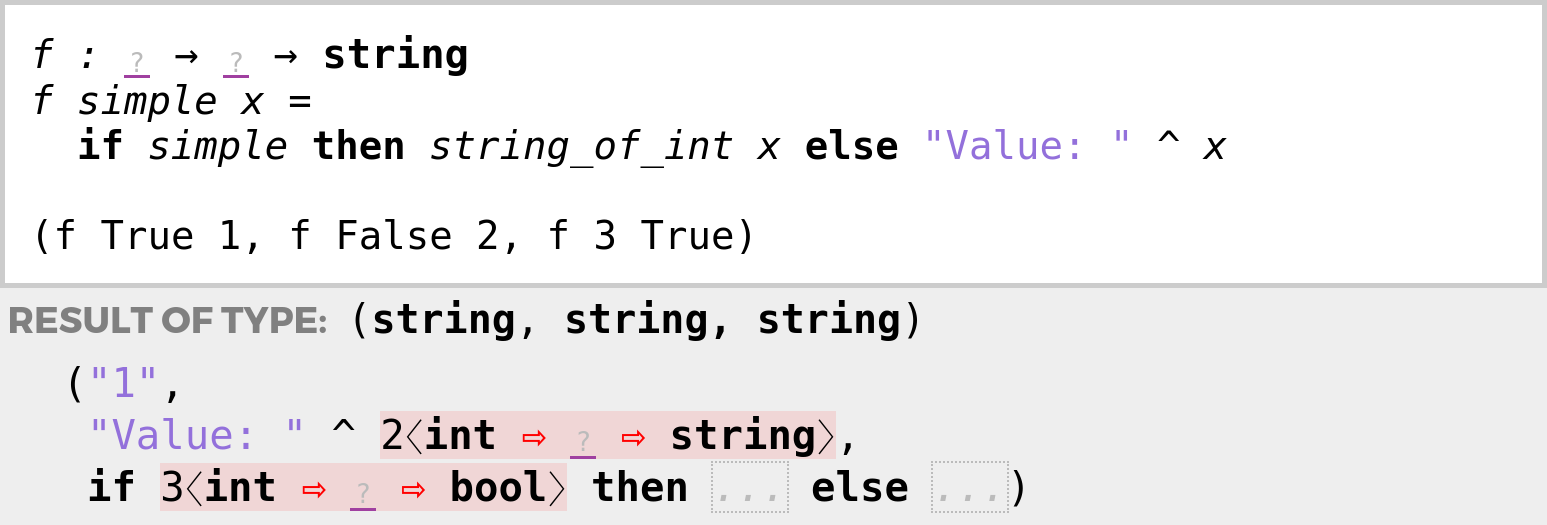
\includegraphics[width=0.71\textwidth,interpolate=false,valign=t]{images/cast-errors.png}
% 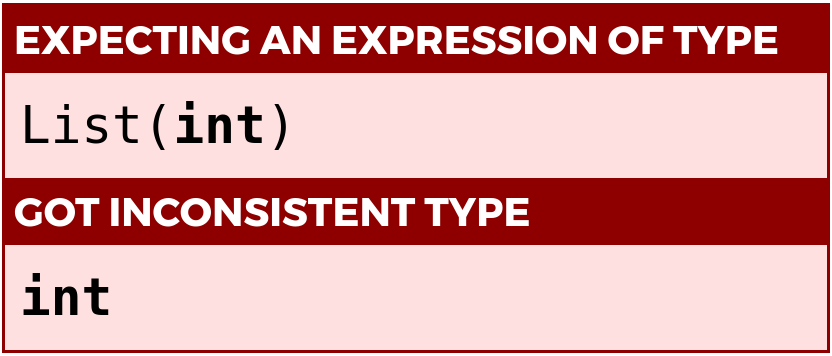
\includegraphics[width=0.28\textwidth,interpolate=false,valign=t]{images/type-inconsistency.png}
\caption{Example 4: Type Holes and Dynamic Type Errors}
\label{fig:cast-errors}
\vspace{-6px}
\end{figure}
% \end{subfigure}


% So far, we have only discussed incomplete programs where a hole appears within an expression.
In \Hazel, the program can also be incomplete because holes appear in types. 
\citet{popl-paper} confirmed that the literature on \emph{gradual type systems} \cite{Siek06a,DBLP:conf/snapl/SiekVCB15} is directly relevant to the problem of reasoning with type holes, by identifying the type hole with the unknown type. 
% Unsurprisingly, then, it is also relevant to the problem of running 
% programs with type holes. 
Indeed, the purpose of gradual typing is to be able to run programs that are not yet sufficiently annotated with types by inserting \emph{casts} only where necessary. As such, let us consider only a small synthetic example to demonstrate what is unique to our approach.

Fig.~\ref{fig:cast-errors} defines a simple function, \li{f}, of two arguments. 
The type annotation on the first line leaves the type of those arguments unknown. 
As such, the \Hazel type system, following the gradual typing approach,
allows the body of the function to use those two
arguments at any type (that is, the hole type is universally consistent). 
Here, the first argument, \li{simple}, is used at one type, \li{bool}, 
and the second argument, \li{x}, is used at two different types in the two branches (perhaps because the programmer made a mistake), 
 \li{int} and  \li{string}  ( \li{^} is string concatenation).
Although \Hazel supports only local type inference as of this writing, 
a system that uses ML-style type reconstruction to fill type holes statically, like GHC Haskell, would only be able to fill the first hole. Leaving the second hole unfilled is 
a parsimonious alternative to arbitrarily or heuristically choosing one of the possibilities and marking the
other uses of \li{x} as ill-typed (see \cite{DBLP:journals/jfp/ChenE18}).

At the bottom of the cell in Fig.~\ref{fig:cast-errors}, we have three 
example applications of \li{f}, tupled together for concision. All three are statically
well-typed, again because the hole type is universally consistent. 
The result at the bottom of Fig.~\ref{fig:cast-errors} demonstrates that the first application
of \li{f} is dynamically unproblematic. This allows the programmer to confirm that 
the first branch operates as intended without the need to 
address the typing problems in the other branch \cite{Bayne:2011:ASD:1985793.1985864}. 
% This flexibility is a common motivation for dynamic and gradual languages .

The second application of \li{f}, in contrast, causes a dynamic type error because the second argument, \li{2}, is an \li{int} but evaluation takes the branch where it is used as a \li{string}. 
Rather than aborting evaluation when this occurs, as in existing gradual type systems, the problematic term becomes a \emph{failed cast} term, shown shaded in red, which can be read ``\li{2} is an \li{int} that was used through a variable of hole type (\li{?}) as a \li{string}''. 
A failed cast acts much like a non-empty hole as a membrane around a problematic term. The surrounding concatenation operation becomes indeterminate, but  
evaluation can continue on to the third application of \li{f}, which is also problematic, this time because the first argument is not a \li{bool} (perhaps because the programmer had an incorrect understanding of the argument order). 
Again, this causes a failed cast to appear, this time in guard position. Like a hole in guard position, evaluation cannot determine which branch to take so the whole conditional becomes indeterminate. 
The pretty printer
hides the two branches behind ellipses for concision.

\ifarxiv

\else
In this small example, it might have only been a small burden for the programmer to provide the intended types in the signature for \li{f}, but there are situations (e.g. during rapid prototyping or a live performance) where the programmer might consider the burden more substantial. This approach ensures that dynamic feedback does not exhibit gaps even when there is a dynamic type error.
\fi


\begin{comment}
\emph{Gradual type systems}~(\eg{}~\cite{XXX,XXX,XXX}) can statically accept
programs that would otherwise be rejected by static type systems---either
because type inference cannot reconstruct a valid type assignment, or because
there may not be a unique valid type assignment at all.
%
In either case, gradual type systems allow types to contain \emph{unknown
types}, and partially unknown types can be used in contexts that require
different types, so long as they are \emph{consistent} (intuitively, equal
modulo the unknown parts).
%
Dynamic casts are then inserted to ensure that these remaining static
discrepancies are not violated at run-time.

\HazelnutLive{} inherits the notion of \emph{type holes} from
\citet{popl-paper}, which serves a similar static purpose as the unknown type in
gradual type systems.
%
In contrast to prior gradually typed languages, however, \HazelnutLive{} can
evaluate ``around'' cast errors in the same way as it does for expression holes.

\overviewExample{3}{Dynamically Typed Negation}

Consider the \li{negate} function (adapted from \cite{ChughPOPL2012}), which
cannot be assigned a static type in a conventional type system---either a
bidirectional one, like in \HazelnutLive{}, or one with ML-style,
unification-based inference---because the argument \li{x} is used at type
\li{int} on line \rkc{XXX} and \li{bool} on line \rkc{XXX}.
%
Therefore, the declared type of \li{x} is the hole type \li{??}, which allows
\li{x} to be used at the conflicting types, with each use expanded into an
expression wrapped in a \emph{cast} that will dynamically check for safety.
%
The return type also uses the hole type \li{??}, leading to additional casts in
the expansion.

\begin{lstlisting}
negate : bool -> ?? -> ??
negate b x =
  if b
    then 0 - x     // expanded to: (0 - (x<?? => int>))<int => ??>
    else not x     // expanded to: (not (x<?? => bool>))<bool => ??>

(negate false 1) + 2 + 3 + (negate true 4)
\end{lstlisting}

\noindent
%
As in prior gradually typed languages~\cite{XXX},
evaluating the expression \li{negate false 1} on line \rkc{XXX} leads to
\li{(not (1<int => ??><?? => bool>))<bool => ??>}, where the inner casts
lead to the \emph{cast error} \li{1<?? =/=> bool>} because \li{1} cannot be
safely treated as having type \li{bool}.
%
Unlike in prior gradually typed languages, however, \HazelnutLive{} evaluates
around the cast error, making progress on the \li{2 + 3 + negate false 4}
expression that surrounds the error; the final indeterminate result is
\li{(not (1<?? =/=> bool>))<bool => ??> + 1}.
%
Just like it is useful for static type checkers to report multiple errors, our
approach allows us to report multiple dynamic cast errors, and otherwise make
progress on expressions that do not depend on failed casts.
%
This approach can be incorporated into existing gradually typed languages.
\end{comment}
% \begin{comment}
\subsection{Live Programming for Debugging}

Previous examples highlighted how running different kinds of incomplete
programs---ones with missing expressions, type-inconsistent expressions, or
missing types---can be useful.
%
Our final example demonstrates how expression holes may be useful even for
complete programs, in order to facilitate debugging and program understanding.

%% \overviewExample{6}{\rkc{...}}
%%
%% \rkc{breakpoints, understanding input/output behavior}

\overviewExample{4}{Quicksort}

Consider the following buggy implementation of quicksort, which contains several
errors.
%
The student wants to debug the implementation and so inserts an expression
around the return expression on line \rkc{XXX}, and runs
\li{quicksort [X,X,X,X,X,X]}.

\begin{lstlisting}
quicksort : list('a) -> list('a)
quicksort [] = []
quicksort (x:xs) =
  let (left, right) = span ((>) x) xs in
  let (left', right') = (quicksort left, quicksort right) in
  ? (left' @ [x] @ right) ?
\end{lstlisting}

\noindent
%
Based on the live environment for the initial call, the student notices that the
values in \li{left} are larger than the pivot \li{x}, but \li{left} was intended
to bind smaller values.
%
This suggests that the student got the filtering predicate backwards, so he
replaces it with \li{(<)} on line \rkc{XXX}.
%
After re-running the program and viewing the live output again, \li{left} now
contains smaller values than \li{x}, but not all of them; \li{right} has some
values that are larger and some that are smaller.
%
The student uses type-based search to find other functions, besides \li{span},
of type \li{('a -> bool) -> 'a list -> ('a list, 'a list)} and finds
\li{partition}.
%
It may be easier for the student to simply try the function rather than studying
the documentation, so he edits line \rkc{XXX} to call \li{partition} instead,
re-runs, and observes that both \li{left} and \li{right} now seem to achieve the
intended partitioning.

Despite these two fixes, the result expression is not yet sorted.
%
In particular, the values greater than the pivot \li{x} are not completely
sorted.
%
Viewing the values of bindings of \li{left'} and \li{right'}, the student sees
that both seem to have correct prefixes of sorted lists, but that they are
incorrect after the pivots.
%
This suggests that something may be wrong with the handling of \li{right'}.
%
Indeed, the student takes a look for uses of \li{right'} and sees that line
\rkc{XXX} mistakenly uses \li{right} instead.
%
Making this change and re-running now produces the desired result, built up as a
hole environment tree that shows how all of the recursive results will be
combined by a series of nested appends.
%
Happy with the results of the program, the student removes the hole around the
expression on line \rkc{XXX}, and evaluation can proceed to perform the nested
appends, producing the final sorted result.
%
\autoref{sec:discussion} discusses how debugging tools may be designed to
systematically insert hole expressions in particular places to achieve certain
debugging and program understanding strategies.
%
%% When run on a larger input, this projection of the full evaluation trace shows a
%% nesting structure---which could be rendered as visualization to help
%% understanding, as described in \autoref{sec:discussion}---whose depth is clearly
%% much smaller than the length of the input list; this suggests that the
%% algorithm, indeed, achieves some sort of sublinear complexity, as intended.
%

\begin{lstlisting}
quicksort : list('a) -> list('a)
quicksort [] = []
quicksort (x:xs) =
  let (left, right) = partition ((<) x) xs in
  let (left', right') = (quicksort left, quicksort right) in
  ? (left' @ [x] @ right') ?
\end{lstlisting}
\end{comment}



% \paragraph{Recap}
% %
% In the above four subsections, respectively, we considered programs with:
% %
% (1) empty expression holes,
% %
% (2) non-empty expression holes for ill-typed expressions,
% %
% (3) type holes, and
% %
% (4) non-empty expression holes for well-typed expressions.
% %
% Next, we will formally describe the novel dynamic semantics of \HazelnutLive{}
% that allows programs with combinations of these kinds of incompleteness to be
% evaluated.

% \input{implementation}
\section{Palettes}

% !TEX root = hazel-LIVE2018.tex
\section{Discussion}
\label{sec:discussion}

Although we will not give the details here, we have developed a formal semantics,
mechanized in the Agda proof assistant, that
specifies how to evaluate programs with holes, and that assigns formal meaning to the fill-and-resume operation.

The editor component of this implementation defines a language of structured edit actions, 
based on the \Hazelnut structure editor calculus developed by \citet{popl-paper}, that inserts holes automatically to guarantee that
every editor state has some, possibly incomplete, type. 
The type safety invariant that we establish then guarantees that every editor state has dynamic meaning. Taken together, the result is a full solution to the gap problem, i.e. a proof-of-concept
live functional programming environment that provides rich static and dynamic feedback that never suffers from temporal or perceptive gaps.


Taken together, the result is a full solution to the gap problem: all of \Hazel's
editor services operate free of temporal or perceptive gaps, because every editor state
has non-trivial static and dynamic meaning. The editor services that make use of the 
tracked hole closures, in turn, provide \Hazel programmers with a uniquely 
\emph{live and direct} typed functional programming experience. 


\clearpage
\bibliography{references,all.short,hazel_NSF}

\end{document}
